
\begin{frame}{Content}{}
\tableofcontents
\end{frame}

%-------------------------------------------------------
%-------------------------------------------------------
\section{Introduction}
%-------------------------------------------------------
%-------------------------------------------------------
%%%%%%%%%%%%%%%%%%%%%%%%%%%%%
%         SLIDE             %
%%%%%%%%%%%%%%%%%%%%%%%%%%%%%
\begin{frame}
  \frametitle{Particle physics: today and future}

  \begin{itemize}
  \item The Large Hadron Collider (LHC) is today's largest particle
    accelerator at CERN (European Organisation for Nuclear Research)
    \begin{itemize}
    \item Proton-proton collisions
    \item Center-of-mass energy: $\sqrt{s}=13\,\tev$
    \item Observation of the Higgs boson in 2012
    \end{itemize}

  \item Still open questions in particles physics remain unanswered:
    \begin{itemize}
    \item Full understanding of the Higgs boson
    \item The origin of matter-antimatter asymmetry
    \item Dark matter
    \item Many more questions ...
    \end{itemize}

  \item Several approaches of high-energy particle colliders to
    address the unanswered questions in the post-LHC era:
    \begin{itemize}
    \item proton-proton ($p~p$) colliders
      \\
      \textcolor{Red}{and/or}
      \\
    \item electron-positron ($e^+e^-$) colliders
    \end{itemize}
  \end{itemize}

\end{frame}

%%%%%%%%%%%%%%%%%%%%%%%%%%%%%
%         SLIDE             %
%%%%%%%%%%%%%%%%%%%%%%%%%%%%%
\begin{frame}
  \frametitle{Hadron vs. Lepton colliders $\Rightarrow$ Discovery to Precision}
  
  % \begin{block}{}
  %   \centering
  %   Discovery to Precision
  % \end{block}

  \begin{columns}[t]
    \column{0.5\textwidth}
    \centering
    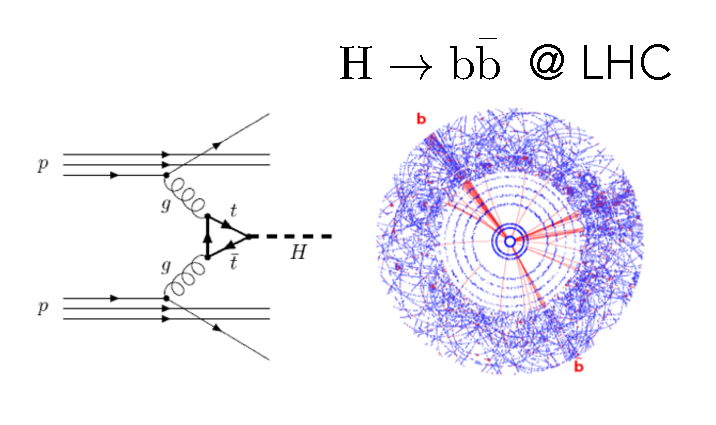
\includegraphics[width=0.6\textwidth]{figures/hadronColliders.pdf}

    \column{0.5\textwidth}
    \centering
    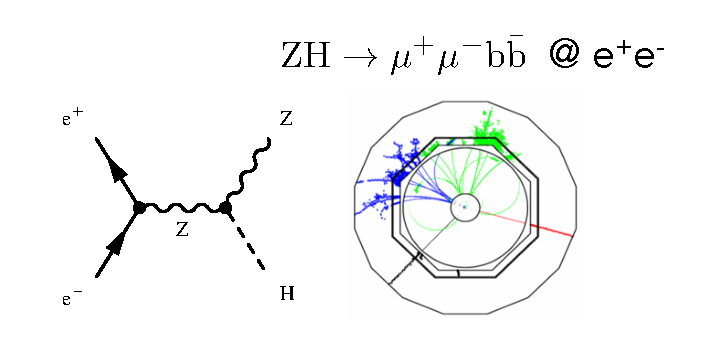
\includegraphics[width=0.6\textwidth]{figures/leptonColliders.pdf}

  \end{columns}


  \begin{columns}[t]
    \column{0.5\textwidth}

    \begin{itemize}
    \item Protons $\Rightarrow$ compound objects
      \begin{itemize}
      \item Unknown event-by-event initial states
      \item Limited achievable precision
      \end{itemize}
    \item High rates of QCD backgrounds
      \begin{itemize}
      \item Complex triggering schemes
      \item High levels of radiation
      \end{itemize}
    \item High cross-sections for coloured-states
    \item High-energy circular pp colliders are feasible
    \end{itemize}

    \column{0.5\textwidth}

    \begin{itemize}
    \item Electrons/positrons $\Rightarrow$ point like
      \begin{itemize}
      \item Well-defined initial states (energy, polarisation)
      \item High-precision measurements
      \end{itemize}
    \item Cleaner experimental environment
      \begin{itemize}
      \item Trigger-less readout
      \item Low levels of radiation
      \end{itemize}
    \item Superior sensitivity for electro-weak states
    \item High-energy $e^+e^-$ collisions ($\geq350\,\gev$) require
      linear colliders
    \end{itemize}

  \end{columns}

\end{frame}


%%%%%%%%%%%%%%%%%%%%%%%%%%%%%
%         SLIDE             %
%%%%%%%%%%%%%%%%%%%%%%%%%%%%%
\begin{frame}
  \frametitle{High-energy $e^+e^-$ colliders studies at CERN}

  \begin{columns}
    \column{0.6\textwidth}
    \begin{itemize}
    \item The Compact LInear Collider (CLIC)
      \begin{itemize}
      \item An $e^{+}e^{-}$ linear collider for the post HL-LHC period.
      \item Energy range $\sqrt{s}$ : \textcolor{blue}{$380\,\gev$} to
        \textcolor{blue}{$3\,\tev$}
        \begin{itemize} 
        \item Two-beam acceleration scheme with gradients of $\sim$100~MV/m.
        \end{itemize}
      \item Precision measurements of:
        \begin{itemize}
        \item Standard Model processes (Higgs, top).
        \item New physics potentially discovered at 13~TeV LHC.
        \item Search for new physics: unique sensitivity to particles with
          electroweak charge.
        \end{itemize}
      \end{itemize}
    \end{itemize}

    \column{0.4\textwidth}
    \begin{tikzpicture}
      \node[anchor=south west,inner sep=0] (image) at (0,
      0){\includegraphics[width=\textwidth]{../figures/CLIC/staging.pdf}};
      \begin{scope}[x={(image.south east)},y={(image.north west)}]
        \node[above, color=white] at (0.5, 0.001) {\textbf{48 km tunnel at 3 TeV stage}};
      \end{scope}
    \end{tikzpicture}
  \end{columns}
  
  \begin{columns}
    \column{0.7\textwidth}

    \begin{itemize}
    \item The Future Circular Collider (FCC-ee):
      \begin{itemize}
      \item Lepton collider in a new 80-100~km tunnel around CERN.
      \item Energy range $\sqrt{s}$: from $90\,\gev$ to $350\,\gev$.
      \item FCC-hh: for proton-proton collisions $\sqrt{s}$ is up to $100\,\tev$.
      \end{itemize}
    \end{itemize}

    \column{0.3\textwidth}
    \centering
    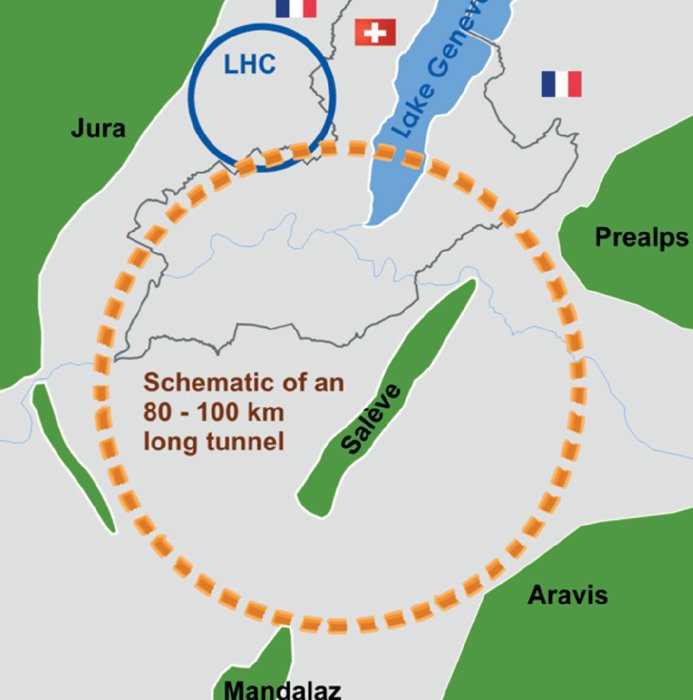
\includegraphics[width=0.9\textwidth]{figures/FCC}

  \end{columns}

\end{frame}


%%%%%%%%%%%%%%%%%%%%%%%%%%%%%
%         SLIDE             %
%%%%%%%%%%%%%%%%%%%%%%%%%%%%%
{
  \usebackgroundtemplate{
    \begin{picture}(100, 265)
      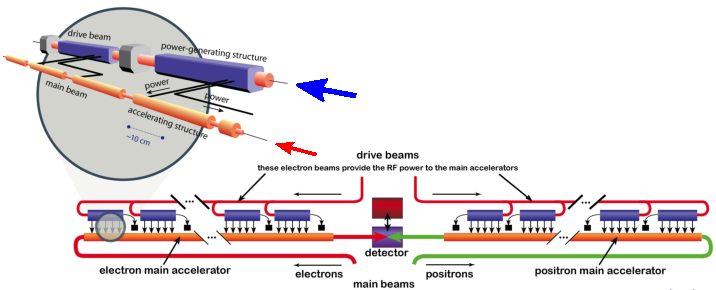
\includegraphics[width=\textwidth]{figures/CLIC_2beam_accel.pdf}
    \end{picture}
  }%
  \begin{frame}
    \frametitle{Two-beam acceleration scheme at CLIC}
    
    \vspace{-1.8cm}
    \begin{itemize}
    \item High-gradient acceleration of \textcolor{Red}{100~MV/m} at
      \textcolor{Red}{12~GHz} \\
      ($\rightarrow$ LHC: 5~MV/m and 400~MHz)
      \begin{itemize}
      \item Limit the length of the accelerator
      \item Traditional klystrons ($\sim$1~GHz) accelerate the drive
        beam (low energy \& high intensity)
      \item Drive beam decelerated $\rightarrow$ energy is fed via an
        RF field in a waveguide to the main beam.
      \end{itemize}
    \end{itemize}
    
    \begin{columns}
      \column{0.5\textwidth}
      \column{0.5\textwidth}
      \begin{itemize}
      \item \textcolor{blue}{Drive beam $\Rightarrow$ RF power}
        \begin{itemize}
        \item 12~GHz bunch structure
        \item High current 100~A
        \item Low energy $2.4\,\gev$ - $240\,\gev$
        \end{itemize}
      \item \textcolor{red}{Main beam $\Rightarrow$ physics}
        \begin{itemize}
        \item Lower current 1.2~A
        \item High energy $9\,\gev$ - $1.5\,\tev$
        \end{itemize}
      \end{itemize}
    \end{columns}

  \end{frame}
}

%%%%%%%%%%%%%%%%%%%%%%%%%%%%%
%         SLIDE             %
%%%%%%%%%%%%%%%%%%%%%%%%%%%%%
\subsection{CLIC beam profile}
\begin{frame}
  \frametitle{Beam profile for CLIC}

 \begin{columns}
   \column{0.6\textwidth}

   \begin{itemize}
   \item Limited train duration due to the duration of the high power levels.
     \begin{itemize}
     \item Bunch crossings (BX): every 0.5~ns.
     \item Train duration: 156~ns (312 bunches).
     \item Train repetition: 20~ms (50~Hz).
     \end{itemize}
   \end{itemize}

   \column{0.4\textwidth}
   \begin{tikzpicture}
     \node[anchor=south west,inner sep=0] (image) at (0,
     0){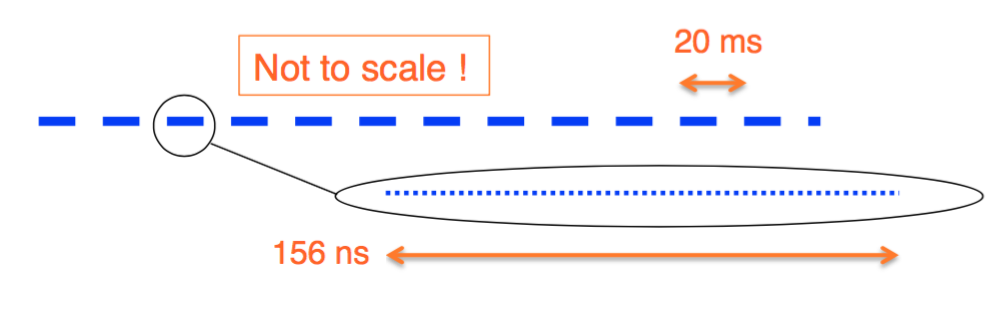
\includegraphics[width=\textwidth]{figures/CLICbeam.png}};
     \begin{scope}[x={(image.south east)},y={(image.north west)}]
       \node[above, color=blue] at (0.5, 0.9) {\textbf{CLIC bunch
           structure}};
     \end{scope}
   \end{tikzpicture}
 \end{columns}
 
 \centering
 \resizebox{0.9\columnwidth}{!}{\begin{tabular}{l c c} 
                                  \toprule 
                                  & CLIC at $\sqrt{s}=3\,\tev$ & LHC at $\sqrt{s}=13\,\tev$\\
                                  \midrule
                                  Instantaneous luminosity $\mathcal{L}$ & $6\times10^{34}$ \inversecmsquaredsec & $1\times10^{34}$ \inversecmsquaredsec \\
                                  Bunch-crossing separation & 0.5~ns & 25~ns \\
                                  IP size in x / y / z directions & 45~nm / 1~nm / $44\,\micron$ & $15\,\micron$ / $15\,\micron$ / 50~cm \\
                                  \bottomrule
                                \end{tabular}
}
                              
                              % \column{0.5\textwidth}
                              % \centering



\begin{itemize}
\item \textcolor{Red}{Bunch separation and train duration: drive
    timing resolution requirements for the detectors.}
\item \textcolor{Green}{Very small beam sizes at the interaction
    point} $\Rightarrow$ beam-induced backgrounds
\end{itemize}



\begin{itemize}
\item Short train duration implies:
  \begin{itemize}
  \item triggerless readout of the detectors.
  \item power pulsing: allows to reduce the average power dissipation.
  \end{itemize}
\end{itemize}

\end{frame}


%%%%%%%%%%%%%%%%%%%%%%%%%%%%%
%         SLIDE             %
%%%%%%%%%%%%%%%%%%%%%%%%%%%%%
\begin{frame}
  \frametitle{Beam-induced backgrounds}
  
  \begin{columns}
    \column{0.8\textwidth}
    \begin{itemize}
    \item Backgrounds:
      \begin{itemize}
      \item \textcolor{blue}{$e^{+}e^{-}$ pairs}: low $p_{T}$, forward
        peaked, limits the inner radius of the VXD.
      \item \textcolor{blue}{$\gamma\gamma\rightarrow$hadrons}: larger
        $p_{T}$ particles, main background in the calorimeters and
        trackers.
      \end{itemize}
    \end{itemize}
    
    \column{0.2\textwidth}    
    \centering
    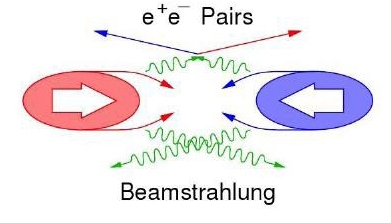
\includegraphics[width=\textwidth]{figures/beamstrahlung.png}
  \end{columns}

  \begin{columns}
    \column{.5\textwidth}    
    \begin{itemize}
    \item Each train consists of:
      \begin{itemize}
      \item At most 1 interesting event.
      \item $>$ 30000 background particles inside the detector.
      \end{itemize}
    \end{itemize}

    \column{0.5\textwidth}
    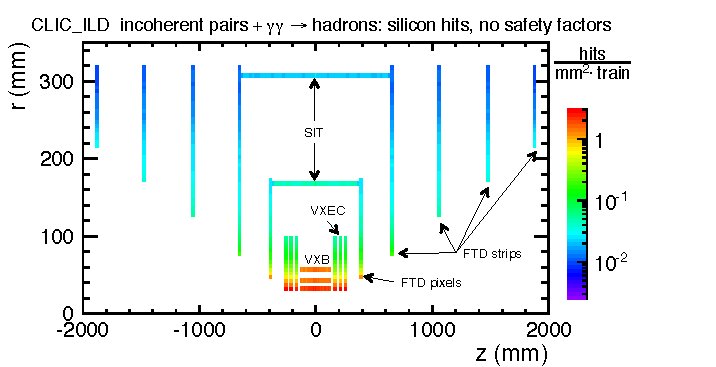
\includegraphics[width=\textwidth]{figures/background_vertex.pdf}
  \end{columns}

  \begin{itemize}
    % \item At most 1 interesting event in each train, $\approx$ 1000 hadronic background events are produced.
  \item Occupancy in the pixel detectors for each train (during \SI{156}{\nano\second}): $\sim$ 3\% for innermost layers.
  \item Radiation exposure of the vertex detector is moderate:
    \begin{itemize}
    \item Total ionising dose (TID): 200~Gy/yr
    \item Non-ionising energy loss (NIEL): $10^{11} n_{eq}/cm^{2}/yr$ (\textcolor{blue}{for ATLAS phase 1: $10^{15} n_{eq}/cm^{2}/yr$})
    \end{itemize}
  \end{itemize}

\end{frame}

%%%%%%%%%%%%%%%%%%%%%%%%%%%%%
%         SLIDE             %
%%%%%%%%%%%%%%%%%%%%%%%%%%%%%
\section{Requirements}
\begin{frame}
  \frametitle{The CLIC detector}

  \begin{columns}
    \column{0.5\textwidth}
    \begin{tikzpicture}
      \node[anchor=south west,inner sep=0] (image) at (0,
      0){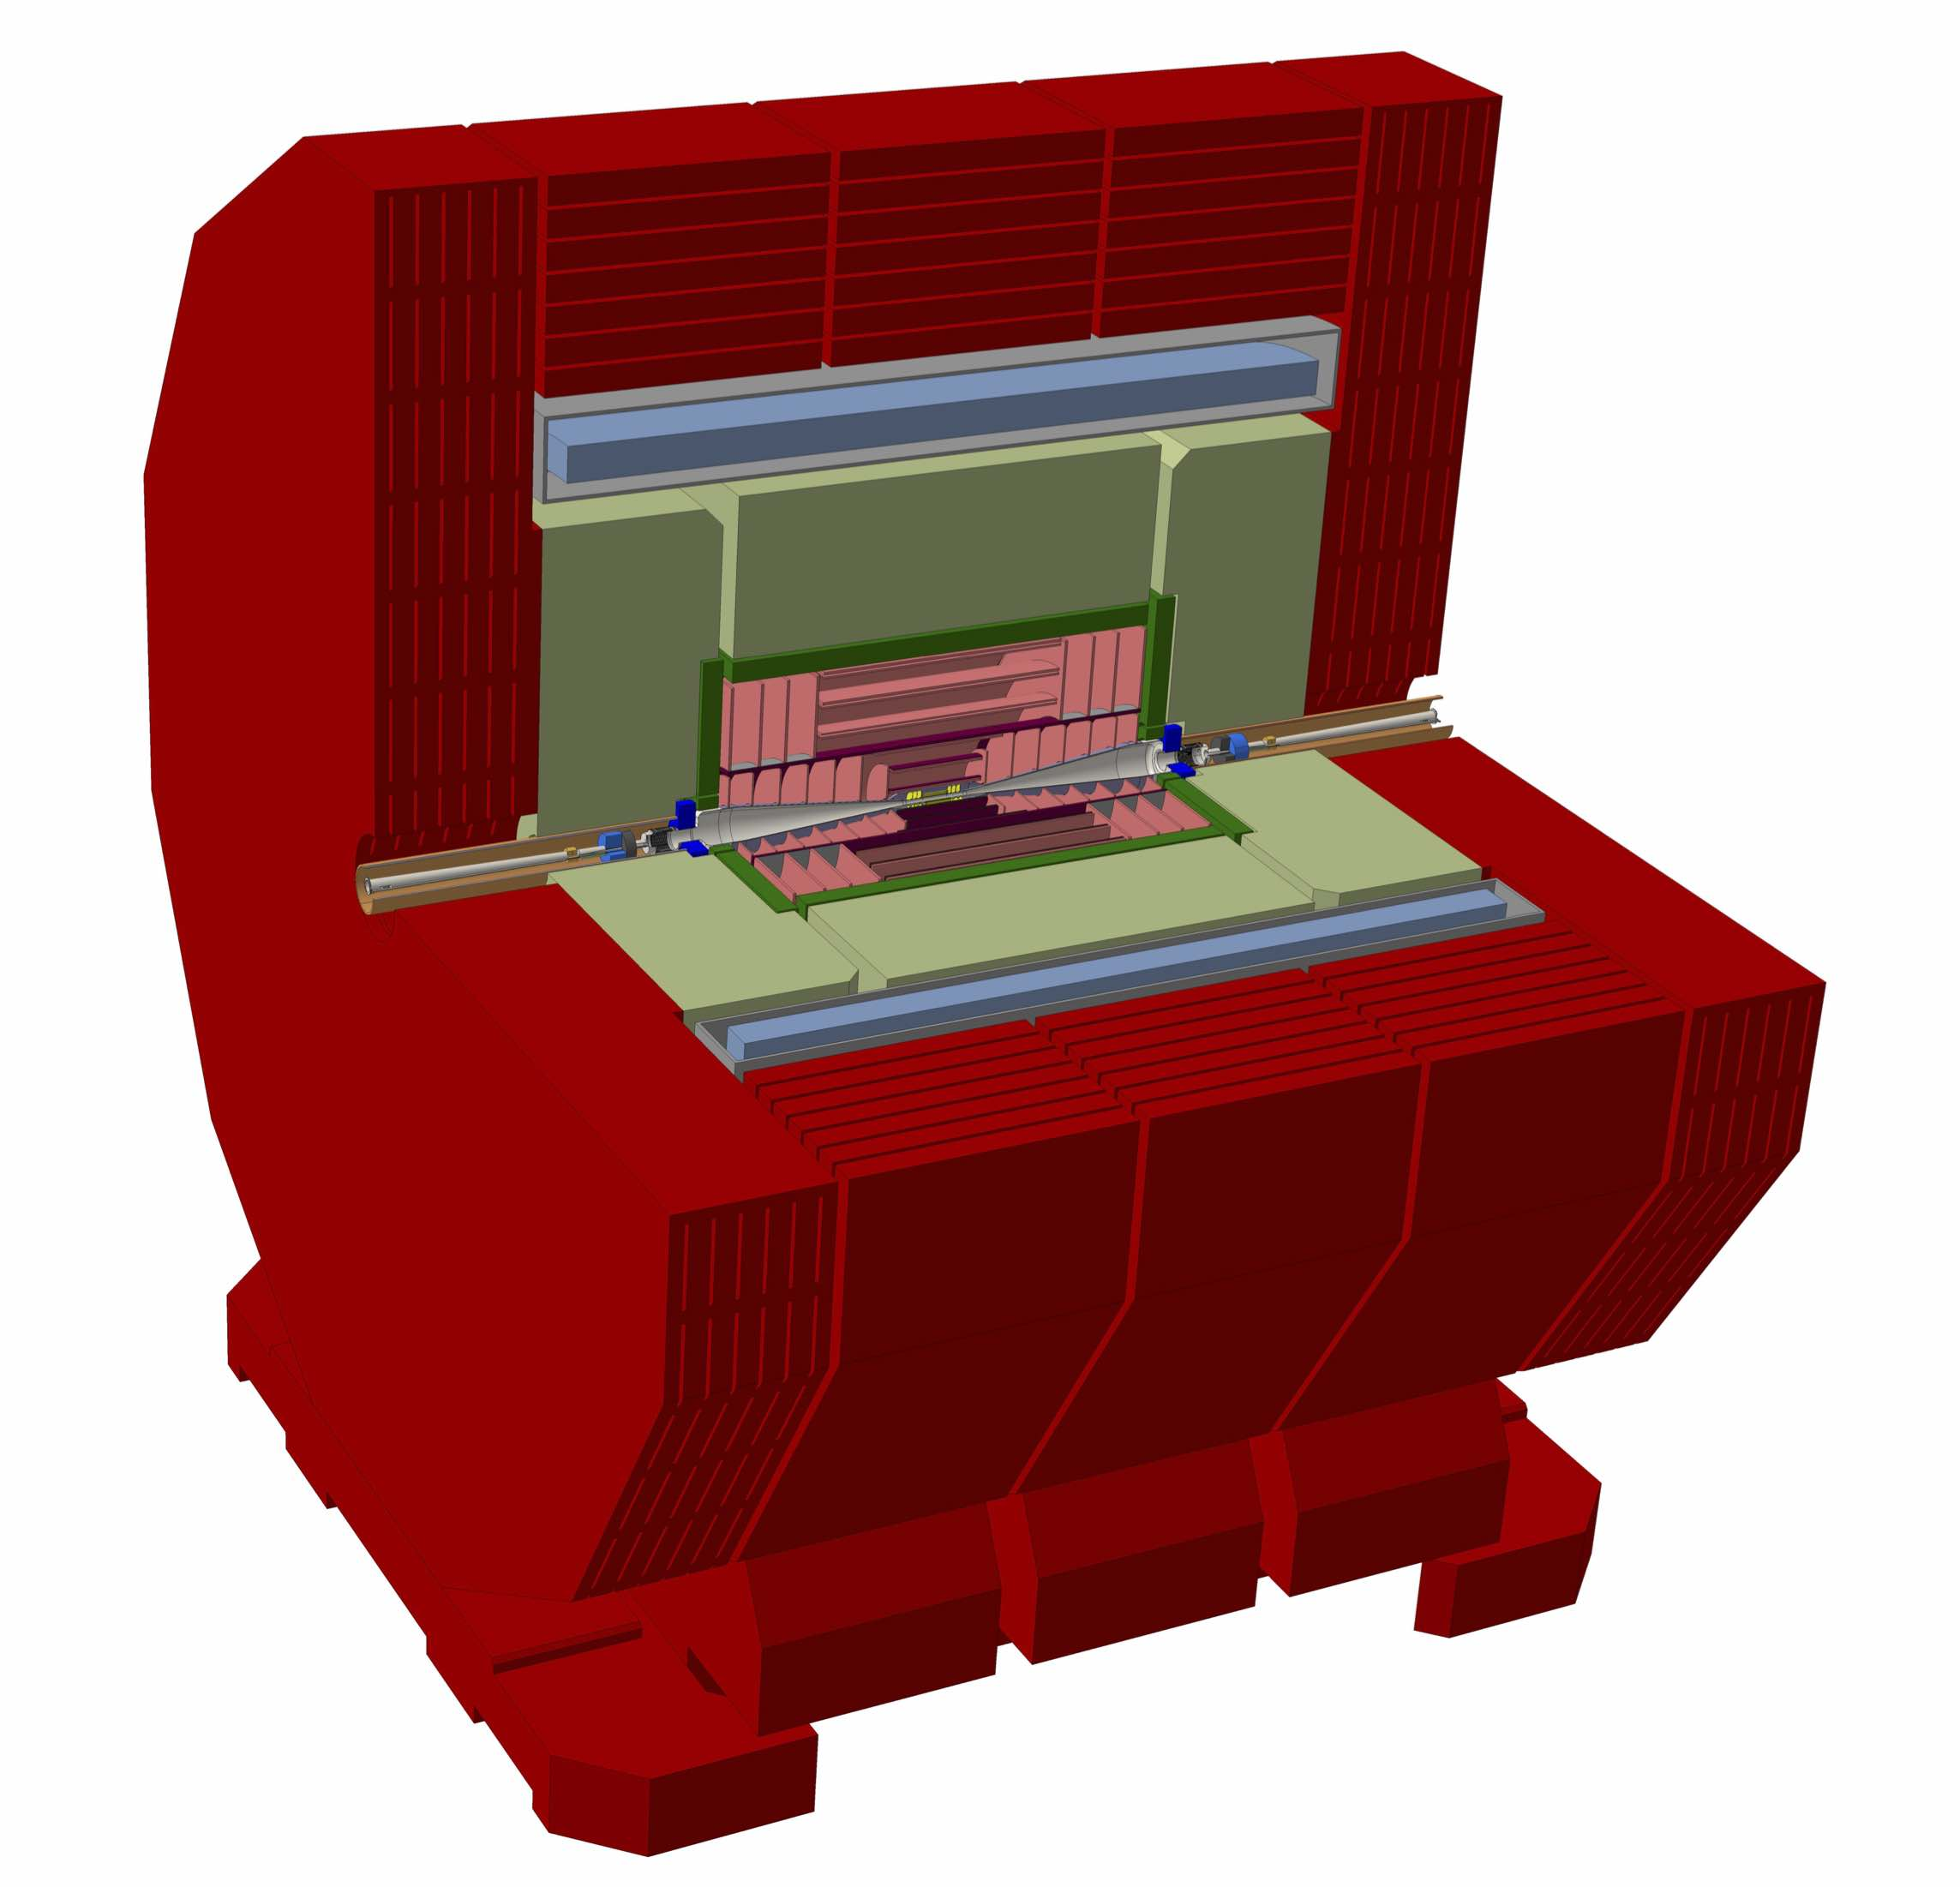
\includegraphics[width=\textwidth]{figures/CLIC_detector_2016.jpg}};
      \begin{scope}[x={(image.south east)},y={(image.north west)}]

        % \draw[help lines,xstep=.1,ystep=.1] (0, 0) grid (1,1);
        % \foreach \x in {0,1,...,9} { \node [anchor=north] at (\x/10,0) {0.\x}; }
        % \foreach \y in {0,1,...,9} { \node [anchor=east] at (0,\y/10)
        %   {0.\y}; }

        \draw[<->,line width=0.5pt] (0.32, 0.0) -- (0.8, 0.13);
        \node[color=black] at (0.6, 0.02) {11.4~m};

        \draw[<->,line width=0.5pt] (0.04, 0.17) -- (0.04, 0.9);
        \node[color=black, rotate=90] at (0.01, 0.5) {12.9~m};
      \end{scope}
    \end{tikzpicture}

    \column{0.5\textwidth}
    \begin{itemize}
    \item CMS-like detector (????? TO BE CHECKED)
    \item Silicon-based and low mass tracking system.
    \item Fine-grained calorimetry system (ECAL and HCAL) optimised
      for particle flow analysis (PFA).
    \item Superconducting solenoid magnet: B=4~T.
    \item Return iron yoke with detectors for muon identification.
    \item Forward region with LumiCal (luminosity monitoring) and
      BeamCal (beam calorimeter).
    \end{itemize}

  \end{columns}

\end{frame}

%%%%%%%%%%%%%%%%%%%%%%%%%%%%%
%         SLIDE             %
%%%%%%%%%%%%%%%%%%%%%%%%%%%%%
\begin{frame}
  \frametitle{Requirements for the vertex detector}

  \begin{columns}
    \column{0.75\textwidth}
    \begin{itemize}
    \item Efficient tagging of heavy quarks through a precise
      determination of displaced vertices can be achieved by: 
      \begin{itemize}
      \item Multi-layer VXD: 6 layers in the barrel and 6 disks
      \item B-field: \textcolor{Blue}{4~T}.
      \item Single point resolution of
        \textcolor{Blue}{$\sim$\SI{3}{\micro\meter}}:
        \textcolor{Blue}{\SI{25}{\micro\meter}} pixel pitch \& analog readout.
      \item Low material budget: $<0.2\%$~X\textsubscript{0}/layer and beam-pipe
        \begin{itemize}
        \item forced airflow cooling \& low-power electronics
          ($\approx 50$~mW/cm\textsuperscript{2})
        \end{itemize}
      \end{itemize} 
    \end{itemize}

    \column{0.25\textwidth}
    \centering
    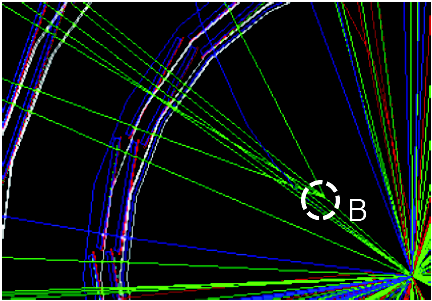
\includegraphics[width=\textwidth]{figures/secondary_vertex.png}

  \end{columns}

  \vspace{-0.3cm}  
  \begin{columns}
    \column{0.6\textwidth}
    \begin{itemize}
    \item Time slicing of \textcolor{Blue}{$\sim$\SI{10}{\nano\second}}
      to reduce the impact of beam-induced backgrounds. \\
      $\Rightarrow$ high-resistive \& depleted sensors, readout with precise timing.
    \end{itemize}

    \column{0.4\textwidth}
    \centering
    \begin{tikzpicture}
      \node[anchor=south west,inner sep=0] (image) at (0,
      0){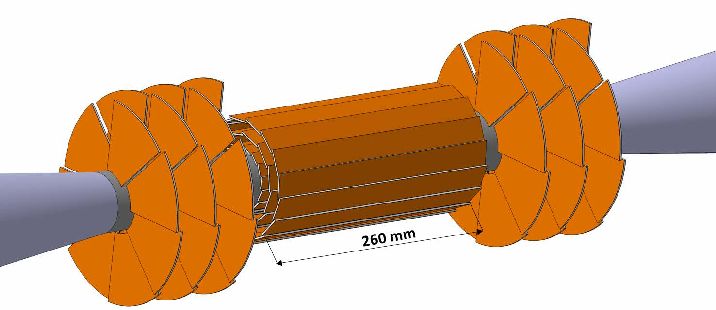
\includegraphics[width=\textwidth]{figures/spiralVXD.pdf}};
      \begin{scope}[x={(image.south east)},y={(image.north west)}]
        \draw[<->, Blue, thick](0.2, 0.0)--(0.84, 0.2);
        \node[below, color=Blue] at (0.5, 0.05) {56 cm};

        % \draw[help lines,xstep=.1,ystep=.1] (0, 0) grid (1,1);
        % \foreach \x in {0,1,...,9} { \node [anchor=north] at (\x/10,0) {0.\x}; }
        % \foreach \y in {0,1,...,9} { \node [anchor=east] at (0,\y/10)
        %   {0.\y}; }

      \end{scope}
    \end{tikzpicture}
  \end{columns}

  % \begin{itemize}
  %   \item Moderate radiation exposure of the vertex detector:
  %     \begin{itemize}
  %     \item Total ionising dose (TID): $<$1~kGy/yr
  %     \item Non-ionising energy loss (NIEL): $10^{11}$~n\textsubscript{eq}/cm\textsuperscript{2}/yr (\textcolor{Blue}{ATLAS phase 1: $10^{15}$~n\textsubscript{eq}/cm\textsuperscript{2}/yr})
  %     \end{itemize}
  % %% \item Time slicing of \textcolor{Blue}{$\sim$\SI{10}{\nano\second}}
  % %%   to reduce the impact of beam-induced backgrounds. \\
  % %%   $\Rightarrow$ high-resistive \& depleted sensors, readout with precise timing.
  % \end{itemize}

\end{frame}

%%%%%%%%%%%%%%%%%%%%%%%%%%%%%
%         SLIDE             %
%%%%%%%%%%%%%%%%%%%%%%%%%%%%%
\begin{frame}
  \frametitle{Flavour-tagging at CLIC}

  \begin{columns}
    \column{0.6\textwidth}
    \begin{itemize}
    \item At $\sqrt{s}=3\,\tev$ the production of the $126\,\gev$
      Higgs
      boson is dominated by the process: \\
      e$^+$e$^- \rightarrow$H$\nu\bar{\nu}$
    \item The Higgs boson decays to b\={b} and c\={c} quark pairs.
    \end{itemize}

    \column{0.4\textwidth}
    \centering
    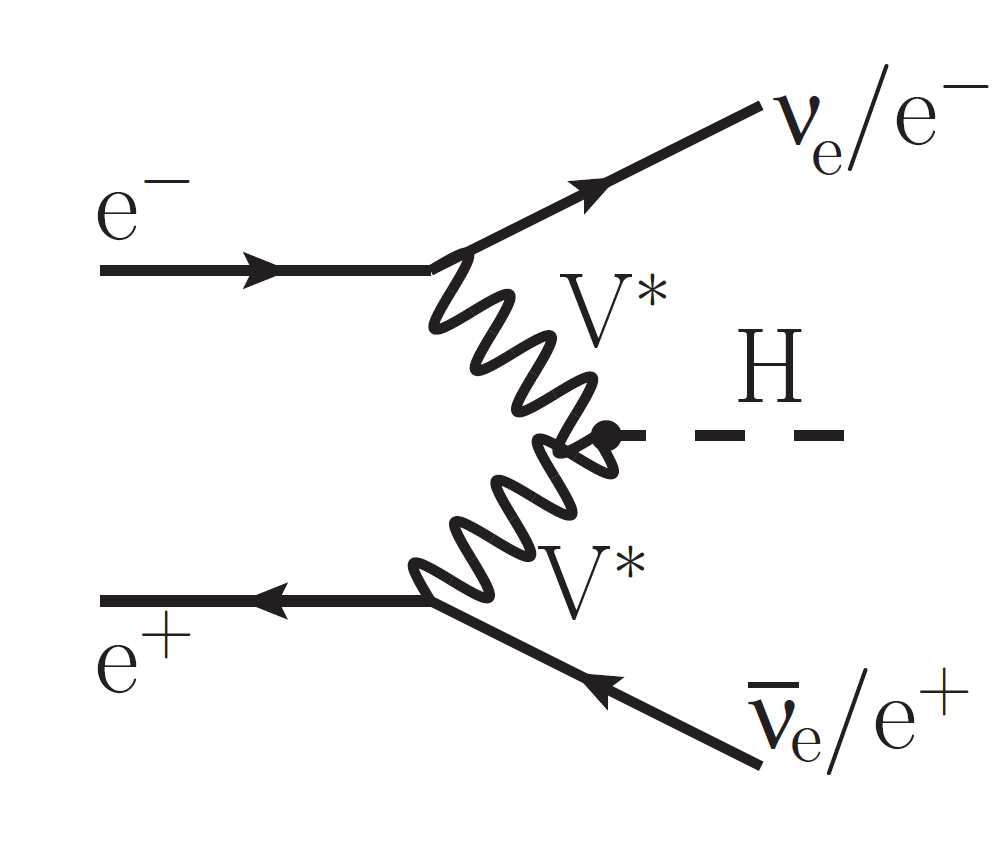
\includegraphics[width=0.5\textwidth]{figures/feynman_higgs.png}
  \end{columns}

  \begin{itemize}
  \item A high-precision vertex detector allows for beauty and
    charm-tagging and to study such decay modes.
  \end{itemize}

  \begin{columns}
    \column{0.5\textwidth}
    \centering
    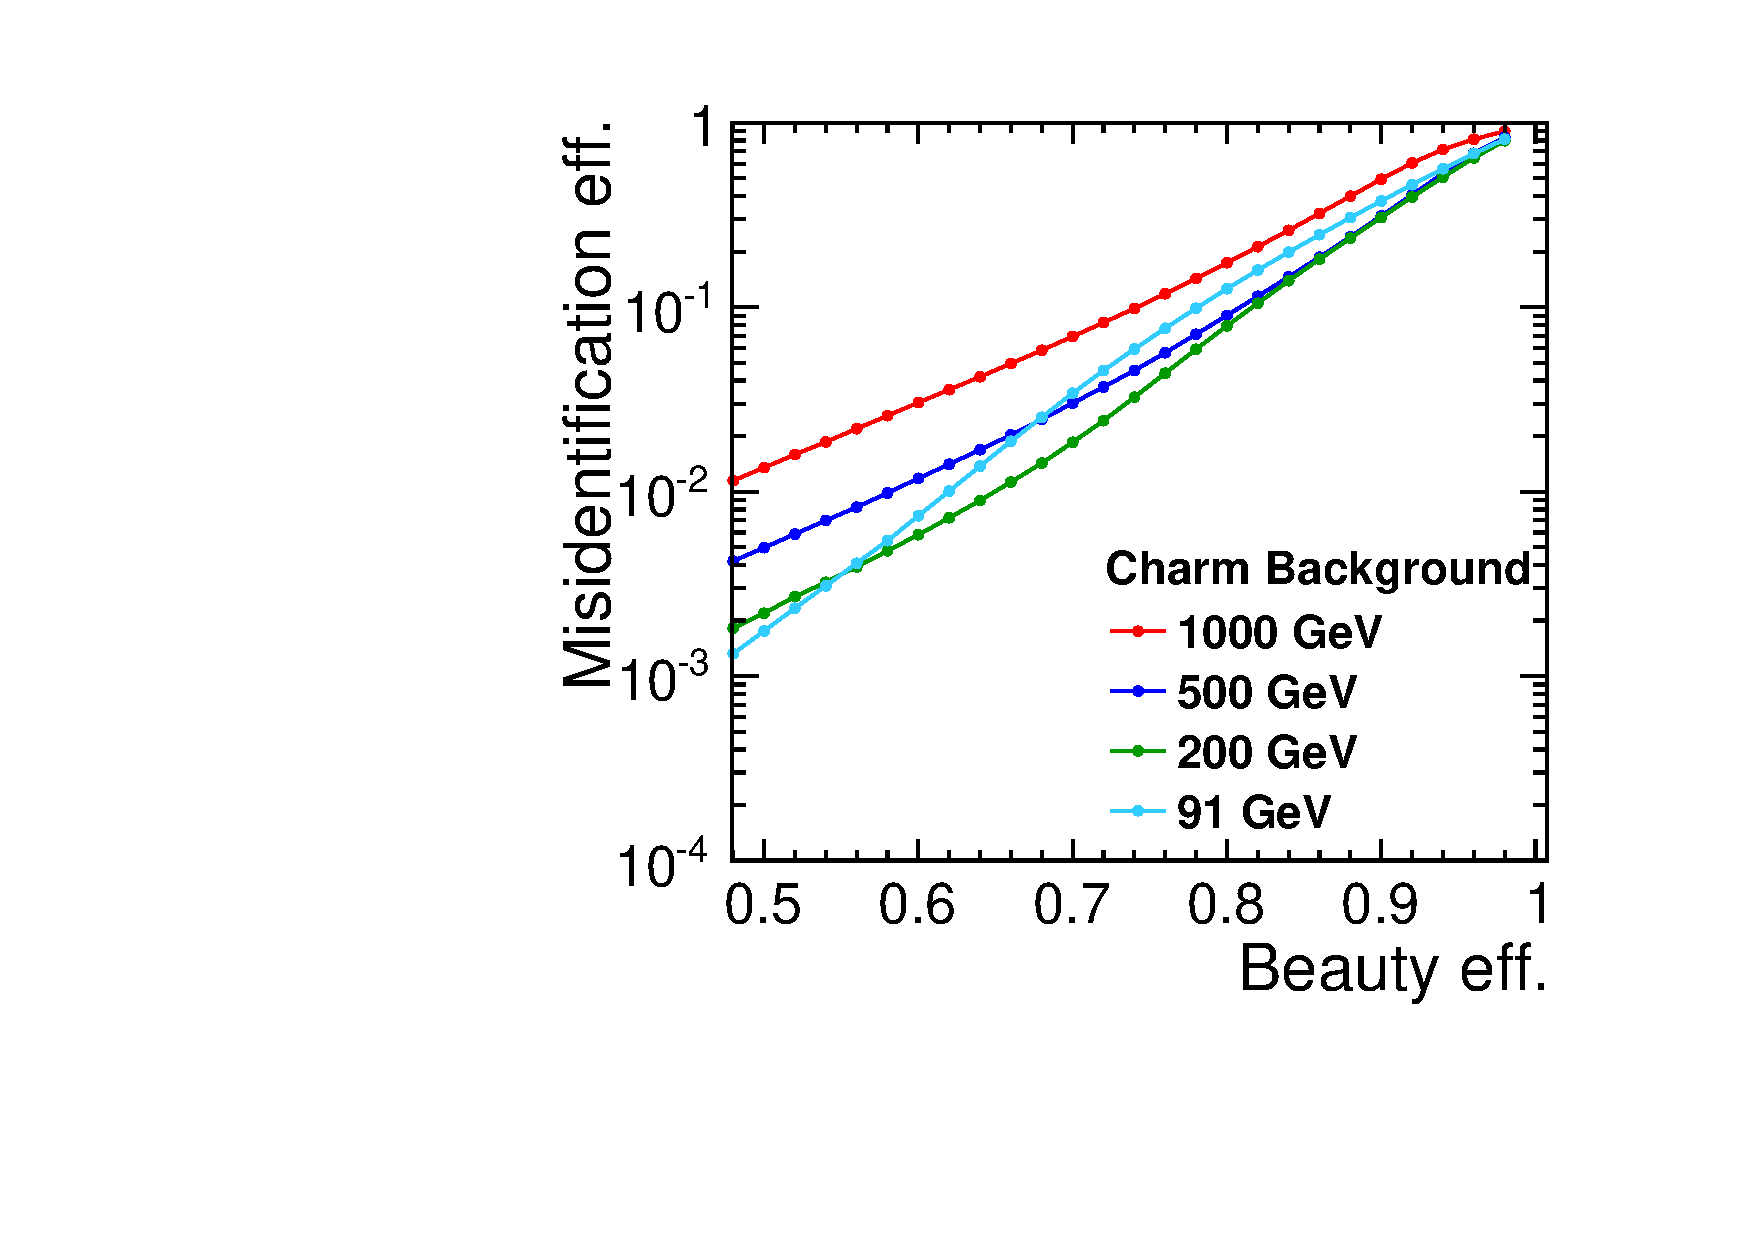
\includegraphics[width=\textwidth]{figures/Global_energies_CLIC_SiD_spirals_Beauty_Charm_.pdf}
    \column{0.5\textwidth}
    \centering
    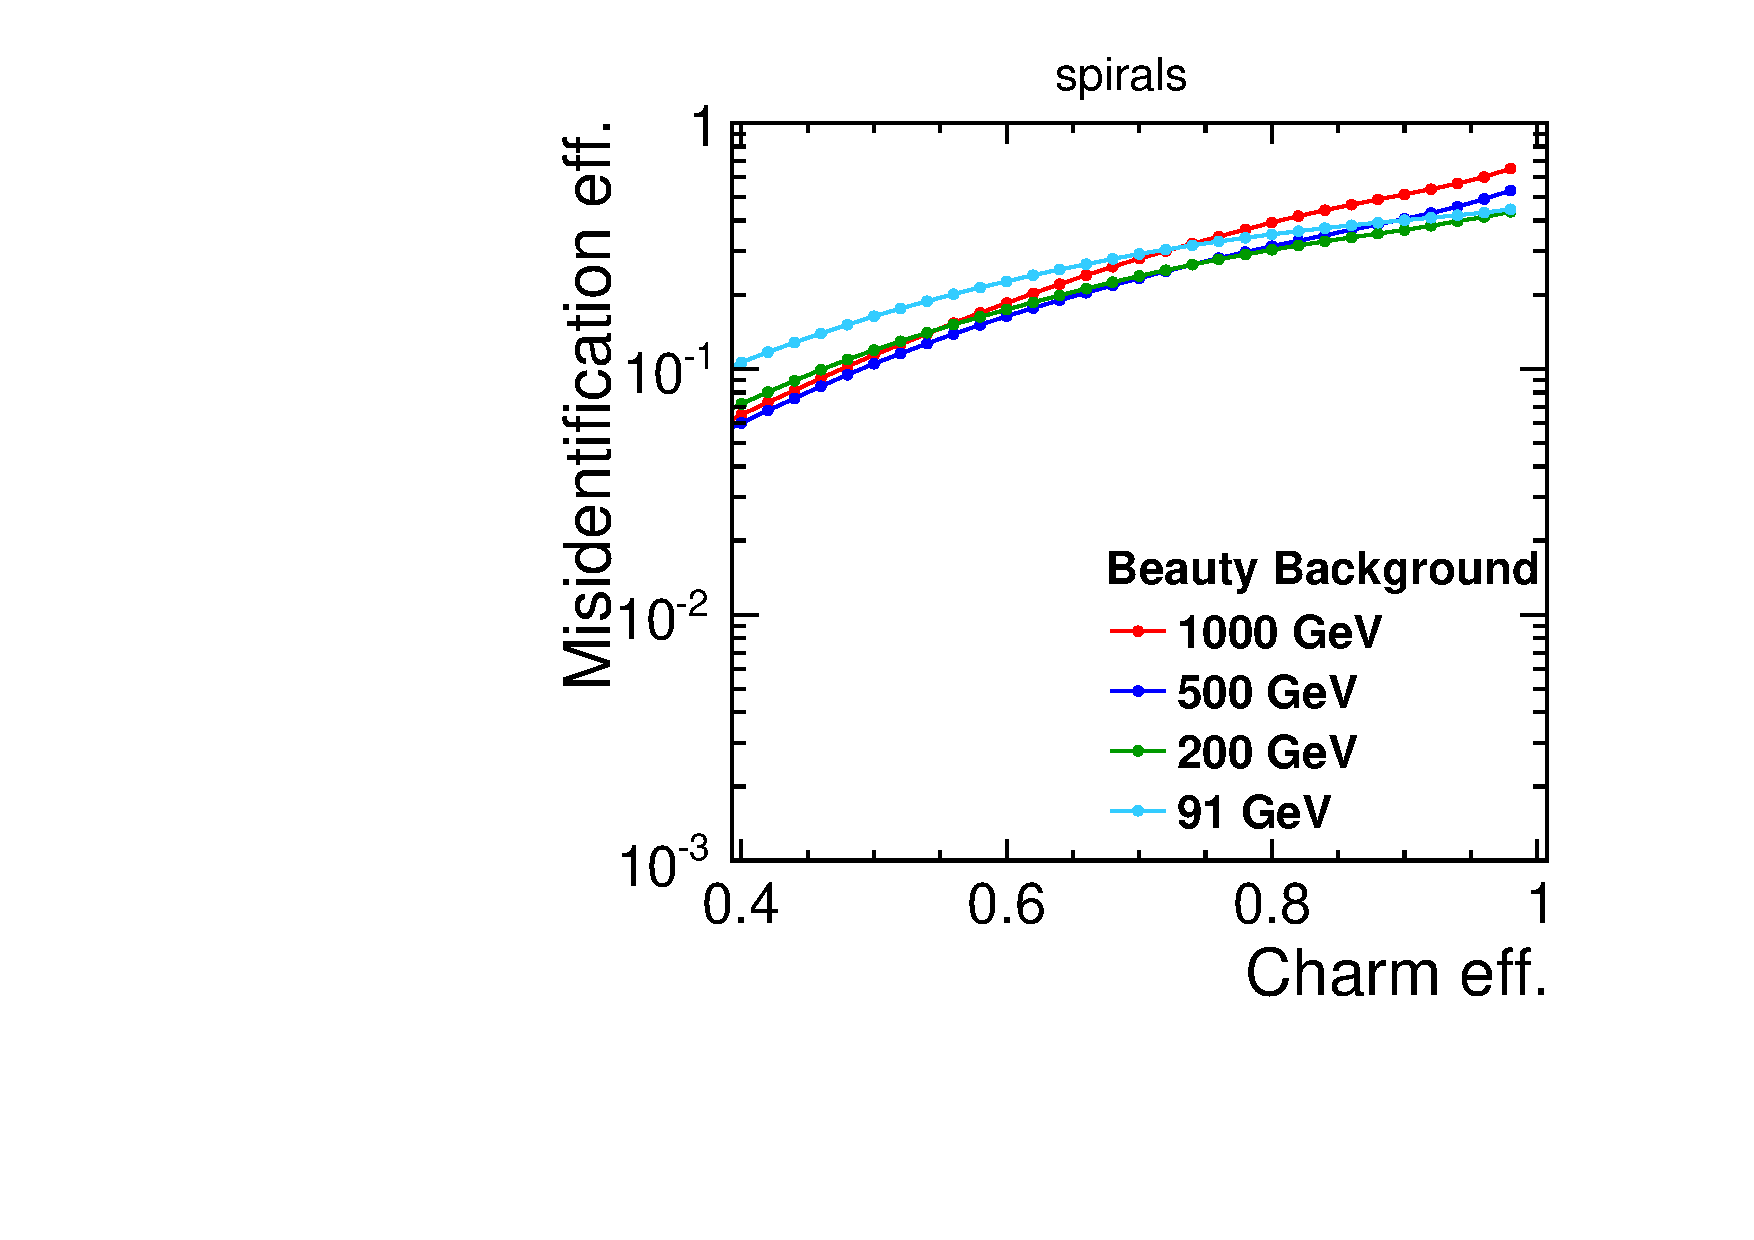
\includegraphics[width=\textwidth]{figures/Global_energies_CLIC_SiD_spirals_Charm_Beauty_.pdf}
  \end{columns}

\end{frame}


%%%%%%%%%%%%%%%%%%%%%%%%%%%%%
%         SLIDE             %
%%%%%%%%%%%%%%%%%%%%%%%%%%%%%
% ----------------------------- %
\tikzstyle{block} = [rectangle, draw, text width=5em, text centered, rounded corners, minimum
height=4em]
\usetikzlibrary{backgrounds,fit,decorations.pathreplacing} 

% ----------------------------- %
\begin{frame}
  \frametitle{R\&D for hybrid pixel detectors at CLIC}

  \begin{itemize}
  \item Hybrid pixel detector: \textcolor{Green}{sensor} \& \textcolor{blue}{readout ASIC}
  \end{itemize}

  \centering
  \begin{adjustbox}{max totalsize={.9\textwidth}{.7\textheight},center}
    \begin{tikzpicture}[node distance = 2.5cm, auto]
      \begin{scope}[x={(image.south east)},y={(image.north west)}]
        
        \coordinate (input);
        \node [block, right of=input, color=Green] (sens) {Sensor};
        \node [block, right of=sens, color=blue] (preamp) {Preamplifier/ Shaper};
        \node [block, right of=preamp, color=blue] (discr) {Discriminator};
        \node [block, right of=discr, color=blue] (conv) {TOT/TOA counters};
        \coordinate[right of=conv] (output);
        
        \draw[arrows=->] (input) -- node [text
        width=4cm,midway] {Incident radiation} (sens);
        \draw[arrows=->] (sens) -- (preamp);
        \draw[arrows=->] (preamp) -- (discr);
        \draw[arrows=->] (discr) -- (conv);
        \draw[arrows=->] (conv) -- node [text width=1.5cm,midway]
        {Digital data bus} (output);
        
        \draw[decorate,decoration={brace, mirror}, thick] (sens.south) to
        node[below,below] (bracket) {Analogue domain}
        (discr.south);
        
        \draw[decorate,decoration={brace, mirror}, thick] (conv.south
        west) to node[below,below] (bracket) {Digital domain} (conv.south
        east);
        
        \draw[decorate,decoration={brace}, thick, color=blue] (preamp.north) to
        node[above, above] (bracket) {Readout chip} (conv.north);
      \end{scope}
    \end{tikzpicture}
  \end{adjustbox}

  \begin{columns}
    \column{0.6\textwidth}
    \begin{itemize}
    \item Achieve $3\,\micron$ single-point resolution with:
      \begin{itemize}
      \item Low material: $50\,\micron$-thick sensor on
        $50\,\micron$-thick ASIC. 
      \item Small pitch: $25\,\micron$ pixel pitch.
      \end{itemize}
    \end{itemize}

    \column{0.4\textwidth}
    \centering
    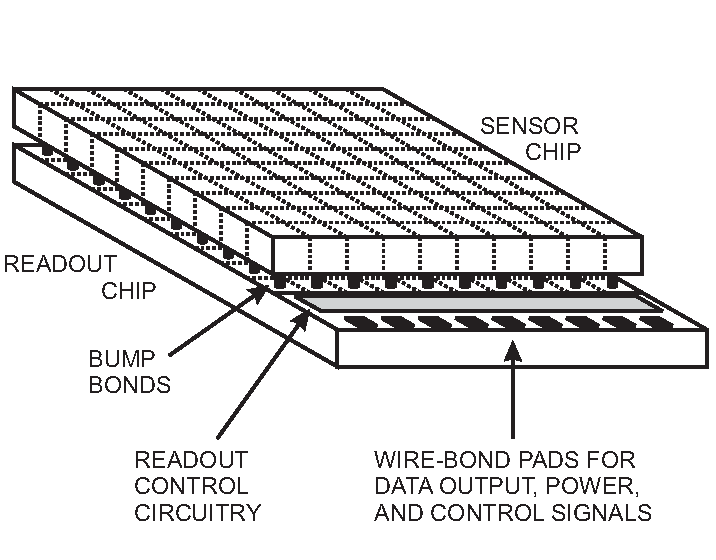
\includegraphics[width=\textwidth]{figures/hybridDet.pdf}
  \end{columns}

  \begin{itemize}
  \item Thin-sensors R\&D:
    \begin{itemize}
    \item The feasibility of thin sensors studied using the Timepix3
      readout ASIC with \textcolor{Red}{$55\,\micron$} pixel pitch.
    \item Use simulations to extrapolate to pixels with a pitch of
      \textcolor{Red}{$25\,\micron$}.
    \end{itemize}
  \end{itemize}

\end{frame}


%%%%%%%%%%%%%%%%%%%%%%%%%%%%%
%         SLIDE             %
%%%%%%%%%%%%%%%%%%%%%%%%%%%%%
\begin{frame}
  \frametitle{The Timepix3 readout chip}

  \begin{columns}
    \column{0.6\textwidth}
    \begin{itemize}
    \item Matrix of $256\times256$ pixels
    \item $55\,\micron$ pixel pitch
      \begin{itemize}
      \item Simultaneous measurement:
      \item Time-of-arrival (TOA) $\Rightarrow$
        \textcolor{Green}{time}
        \item Time-over-threshold (TOT) $\Rightarrow$
          \textcolor{Green}{energy}
      \end{itemize}
    \item Data-driven mode readout:
      \begin{itemize}
      \item Low dead time
      \item High readout rates: 40~Mhits/(s$\cdot$cm\textsuperscript{2})
      \end{itemize}
    \end{itemize}

    \column{0.4\textwidth}
    \centering 
    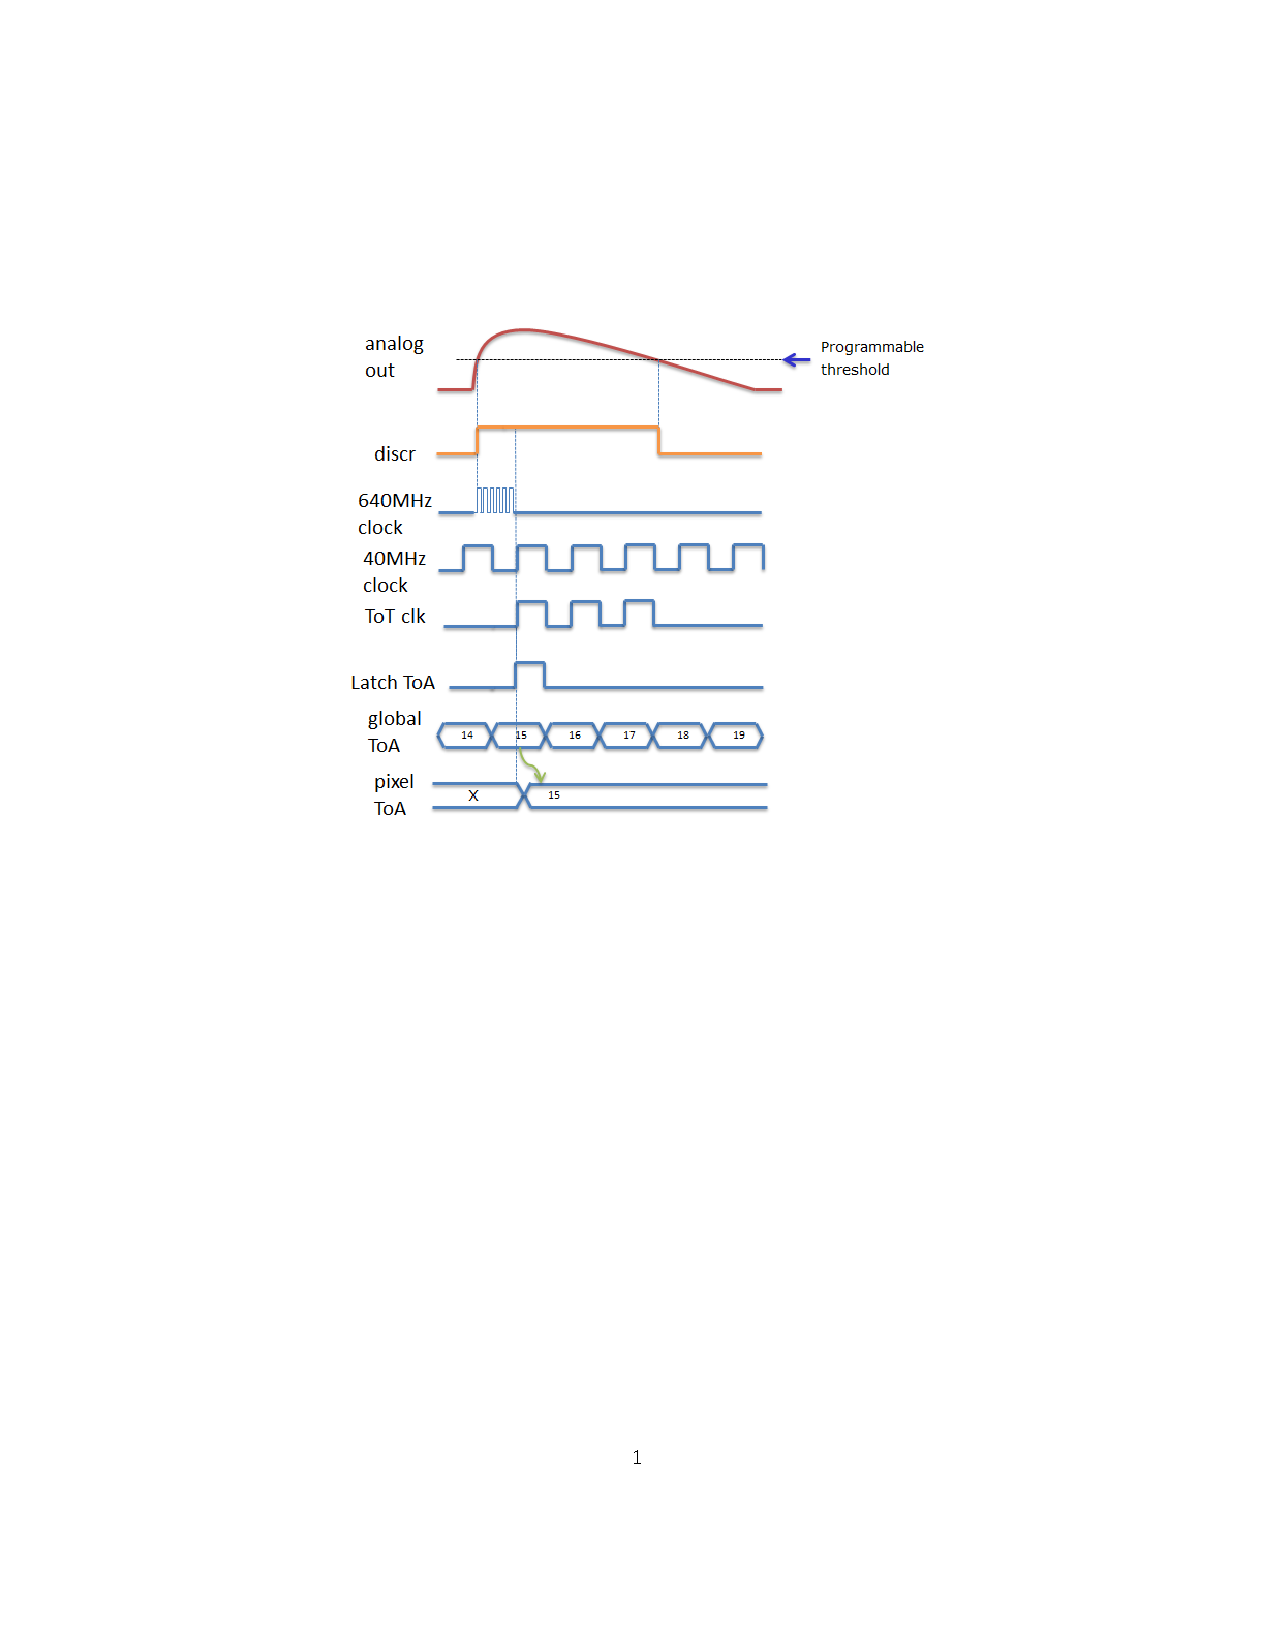
\includegraphics[width=\textwidth, trim = 50mm 140mm
    60mm 50mm, clip]{../figures/Calibration/TOT_TOA_explanation.pdf}
  \end{columns}


  \begin{columns}
    \column{0.5\textwidth}
    \begin{itemize}
    \item TOT - energy calibration:
      \begin{itemize}
      \item Non-linear relationship between the measured TOT and the
        deposited energy.
      \item Internal analogue test pulse generator \\
        Q=C$\cdot \Delta$V
      \end{itemize}
    \item Preferred operation in the linear regime
    \end{itemize}



    \column{0.5\textwidth}
    \centering
    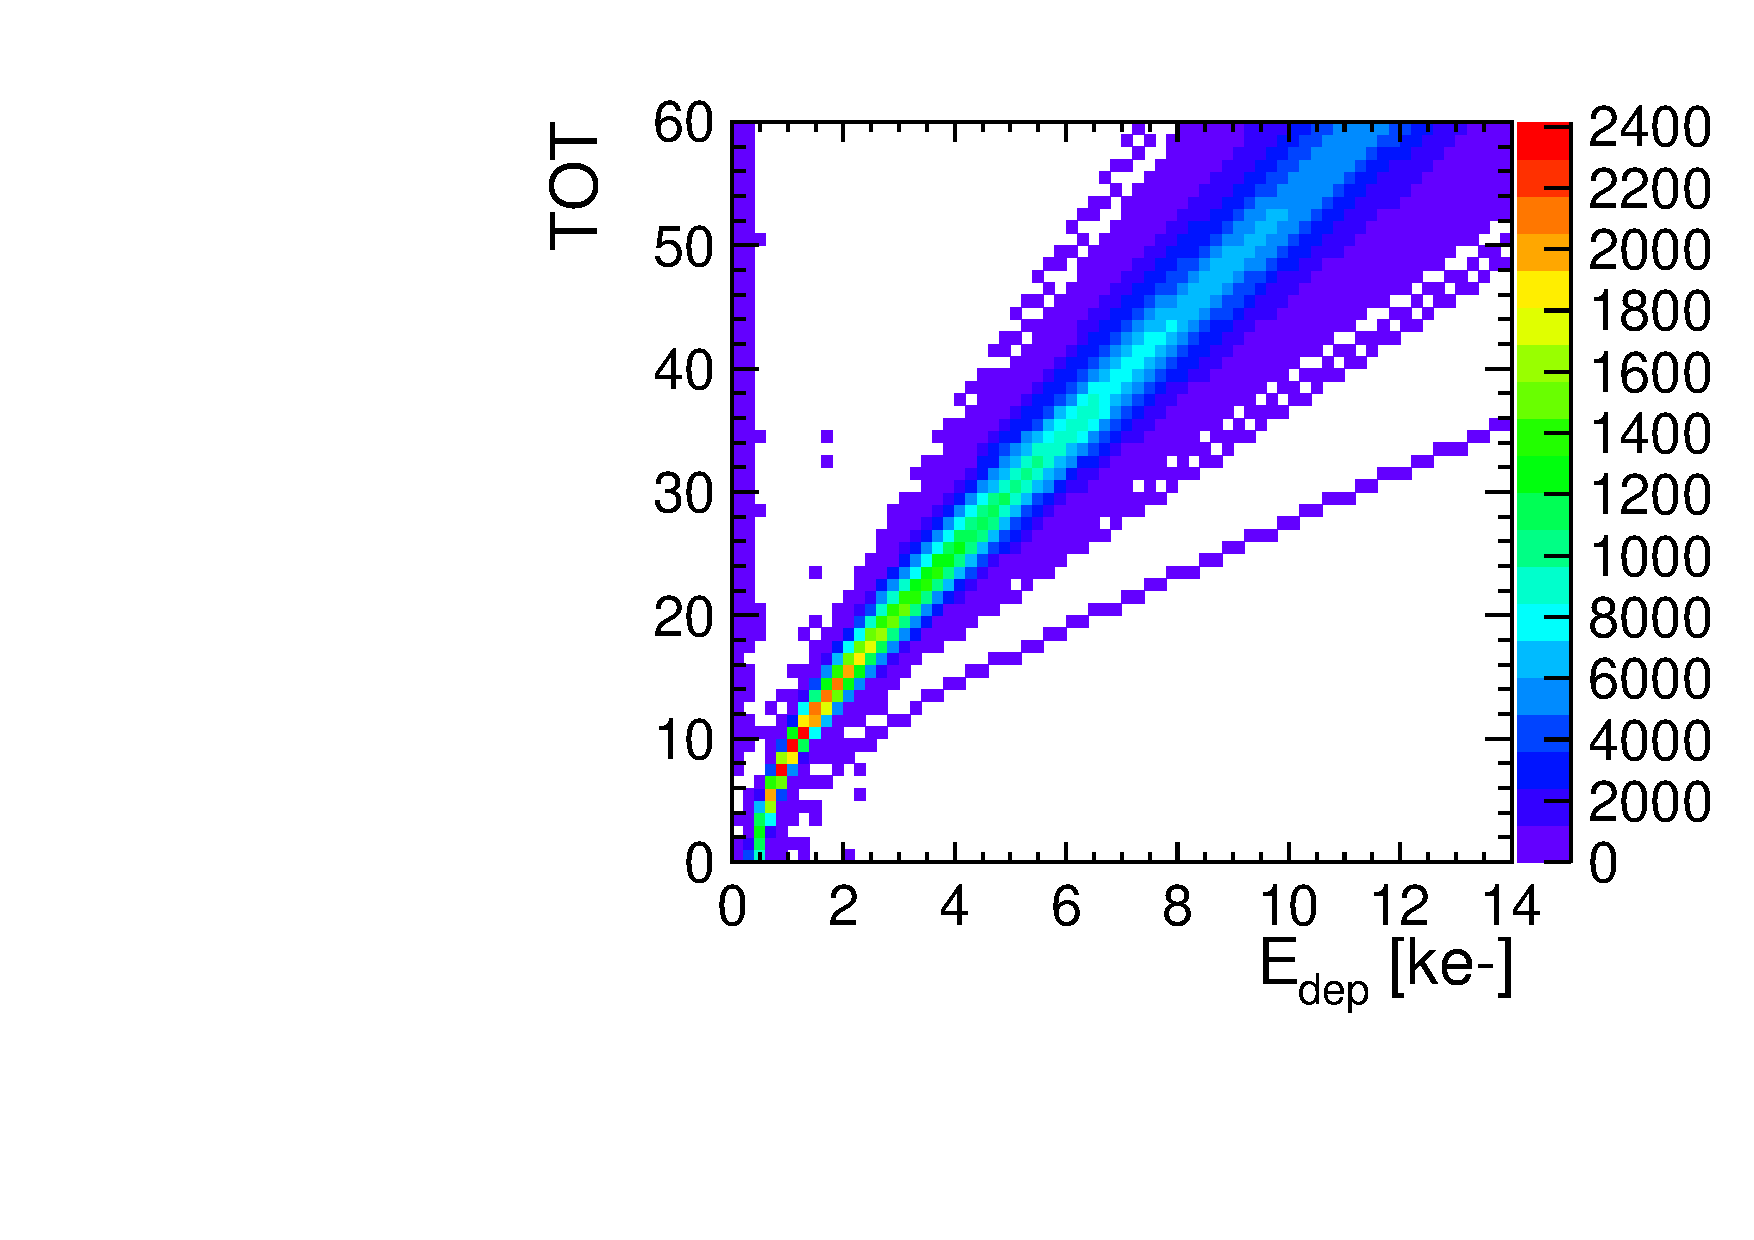
\includegraphics[width=\textwidth]{../figures/Calibration/TOTcalibration_W0005_E02_thresh1160.pdf}
  \end{columns}

\end{frame}

%%%%%%%%%%%%%%%%%%%%%%%%%%%%%
%         SLIDE             %
%%%%%%%%%%%%%%%%%%%%%%%%%%%%%
\begin{frame}
  \frametitle{Test-beam measurements of thin sensors}

  \begin{itemize}
  \item Test-beam campaigns at the CERN SPS with $120\,\gev$ pion
    beam.
  \item CLICpix Timepix3 pixel-beam telescope $\Rightarrow$ track
    reconstruction.
  \end{itemize}


  \begin{columns}
    \column{0.6\textwidth}
    \centering
    \begin{tikzpicture}
      \node[anchor=south west,inner sep=0] (image) at
      (0,0){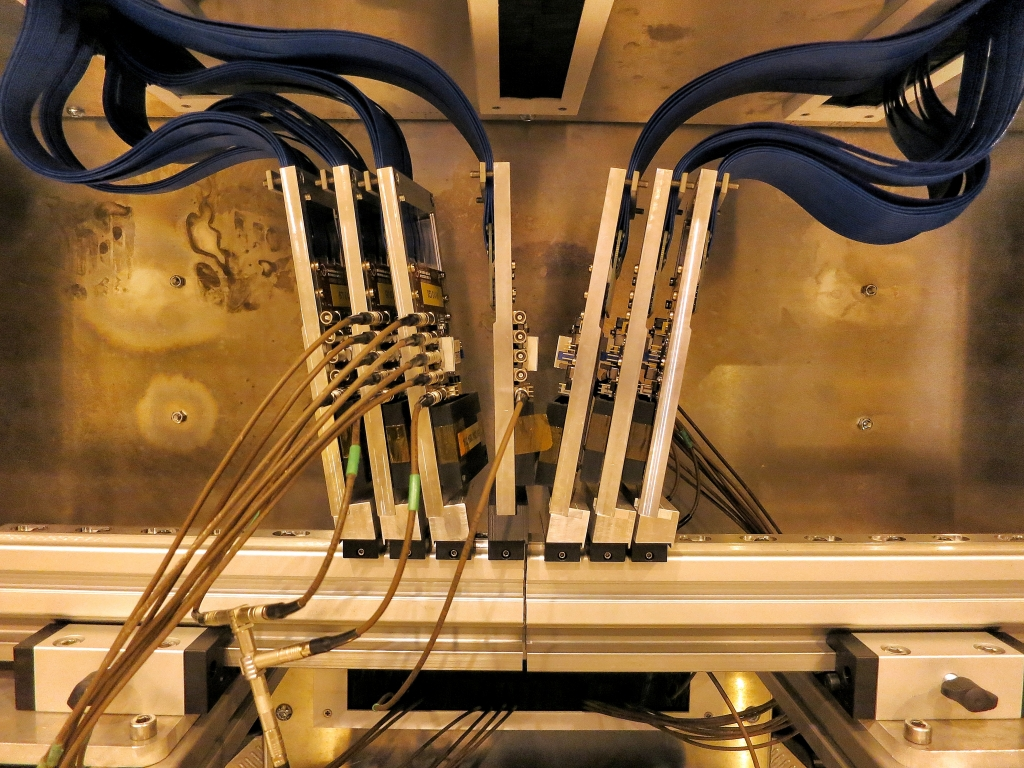
\includegraphics[width=\textwidth]{../figures/ActiveEdge/Timepix3Telescope.jpeg}};
      \begin{scope}[x={(image.south east)},y={(image.north west)}]
        \node[above, color=white] at (0.5, 0.85) {Device Under Test};
        \node[above, color=white] at (0.5, 0.78) {(\textbf{DUT})};

        \draw[->, very thick, color=black](0.75, 0.38) -- (0.25, 0.44);
        % \node[right, color=black] at (0.77, 0.42) {\textbf{Beam}};

        \draw[<->, very thick, color=black](0.33, 0.25) -- (0.66, 0.25);
        \node[below, color=black] at (0.5, 0.25) {\textbf{152~mm}};

        \node[color=black] at (0.64, 0.32) {\textbf{0}};
        \node[color=black] at (0.6, 0.32) {\textbf{1}};
        \node[color=black] at (0.55, 0.32) {\textbf{2}};

        \node[color=black] at (0.44, 0.32) {\textbf{3}};
        \node[color=black] at (0.39, 0.32) {\textbf{4}};
        \node[color=black] at (0.35, 0.32) {\textbf{5}};
        

        \node[circle, fill, color=Red, inner sep=0pt, minimum size=4pt]
        at (0.64, 0.4) {}; 
        \node[circle, fill, color=Red, inner sep=0pt, minimum size=4pt]
        at (0.6, 0.4) {};
        \node[circle, fill, color=Red, inner sep=0pt, minimum size=4pt]
        at (0.55, 0.4) {};
        \node[circle, fill, color=Red, inner sep=0pt, minimum size=4pt]
        at (0.42, 0.42) {};
        \node[circle, fill, color=Red, inner sep=0pt, minimum size=4pt]
        at (0.37, 0.43) {};
        \node[circle, fill, color=Red, inner sep=0pt, minimum size=4pt]
        at (0.32, 0.43) {};

        \node[star, fill, color=Green, inner sep=0pt, minimum size=8pt]
        at (0.49, 0.41) {};

        % \draw[help lines,xstep=.1,ystep=.1] (0, 0) grid (1,1);
        % \foreach \x in {0,1,...,9} { \node [anchor=north] at (\x/10,0) {0.\x}; }
        % \foreach \y in {0,1,...,9} { \node [anchor=east] at (0,\y/10) {0.\y}; }
        
      \end{scope}
    \end{tikzpicture} 
    \\
    
    \begin{tikzpicture}
      \begin{scope}[x={(image.south east)},y={(image.north west)}]

        % \draw[help lines,xstep=.1,ystep=.1] (0, 0) grid (1,1);
        % \foreach \x in {0,1,...,9} { \node [anchor=north] at (\x/10,0) {0.\x}; }
        % \foreach \y in {0,1,...,9} { \node [anchor=east] at (0,\y/10) {0.\y}; }
        
         \node[circle, fill, color=Red, inner sep=0pt, minimum size=4pt]
        at (0.1, 0.9) {};
        \node[right, color=black] at (0.1, 0.9) {: measured track
          position};

        \node[star, fill, color=Green, inner sep=0pt, minimum
        size=8pt] at (0.1, 0.8) {}; \node[right, color=black] at (0.1,
        0.8) {: reconstructed track position};
      \end{scope}
    \end{tikzpicture} 


    \column{0.4\textwidth}

    \begin{itemize}
    \item Pointing resolution on the DUT:
      \textcolor{Green}{$\sim2\,\micron$}
    \item Time resolution per plane: \textcolor{Green}{$\sim$1~ns}
    \end{itemize}

    % \begin{tikzpicture}
    %   \begin{scope}[x={(image.south east)},y={(image.north west)}]

    %     \draw[help lines,xstep=.1,ystep=.1] (0, 0) grid (1,1);
    %     \foreach \x in {0,1,...,9} { \node [anchor=north] at (\x/10,0) {0.\x}; }
    %     \foreach \y in {0,1,...,9} { \node [anchor=east] at (0,\y/10) {0.\y}; }
        
    %   \end{scope}
    % \end{tikzpicture} 

  \end{columns}

\end{frame}


%%%%%%%%%%%%%%%%%%%%%%%%%%%%%
%         SLIDE             %
%%%%%%%%%%%%%%%%%%%%%%%%%%%%%
\begin{frame}
  \frametitle{AllPix simulation framework}

  \begin{columns}
    \column{0.6\textwidth}

    \begin{itemize}
    \item A general purpose pixel-detector simulation framework (in
      C/C++) based on \textsc{Geant4}.
    \item Fully customisable for detector geometry description:
      \begin{itemize}
      \item thickness, pixel-pitch, bump geometry, material
      \end{itemize}
    \item \textcolor{Green}{\textbf{Digitisation}}: responsible for the
      full simulation of the detector including the sensor and the
      readout chip. 
      \begin{itemize}
      \item Defined by the user.
      \item Different for each sensor/ASIC technology.
      \end{itemize}
    \end{itemize}
    
    \column{0.4\textwidth}
    \centering
    \begin{tikzpicture}
      \node[anchor=south west,inner sep=0] (image) at
      (0,0){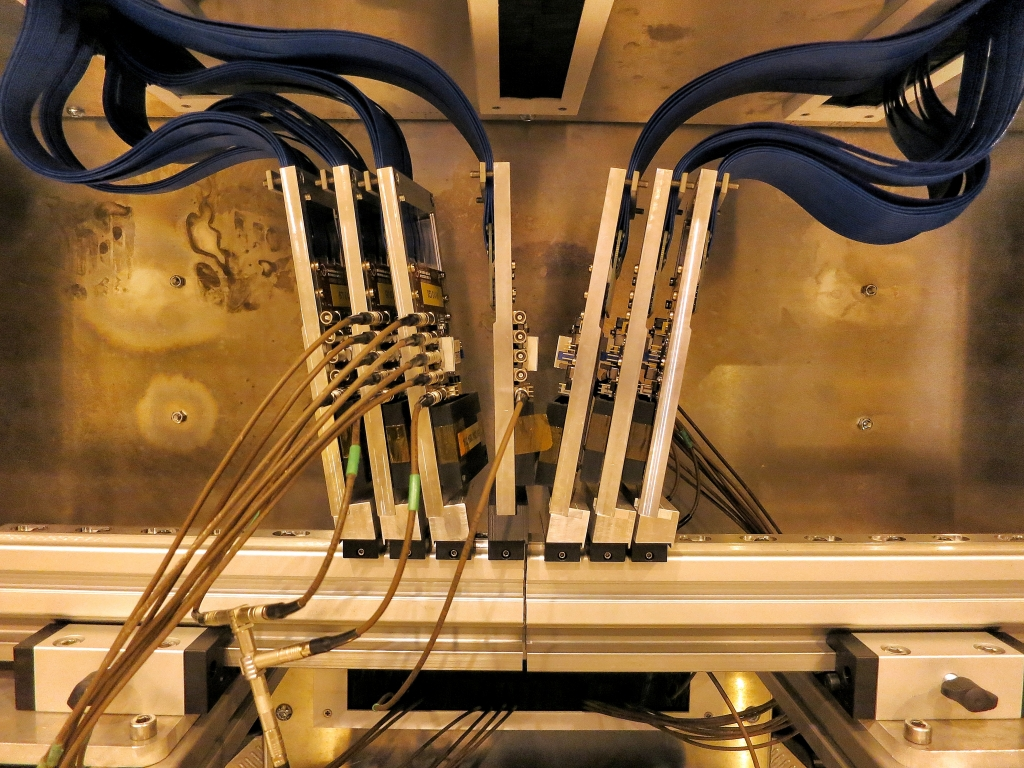
\includegraphics[width=\textwidth]{../figures/ActiveEdge/Timepix3Telescope.jpeg}};
      \begin{scope}[x={(image.south east)},y={(image.north west)}]
        \node[above, color=white] at (0.5, 0.85) {The CLICpix Timepix3
        telescope};
      \end{scope}
    \end{tikzpicture}

    \centering
    \begin{tikzpicture}
      \node[anchor=south west,inner sep=0] (image) at
      (0,0){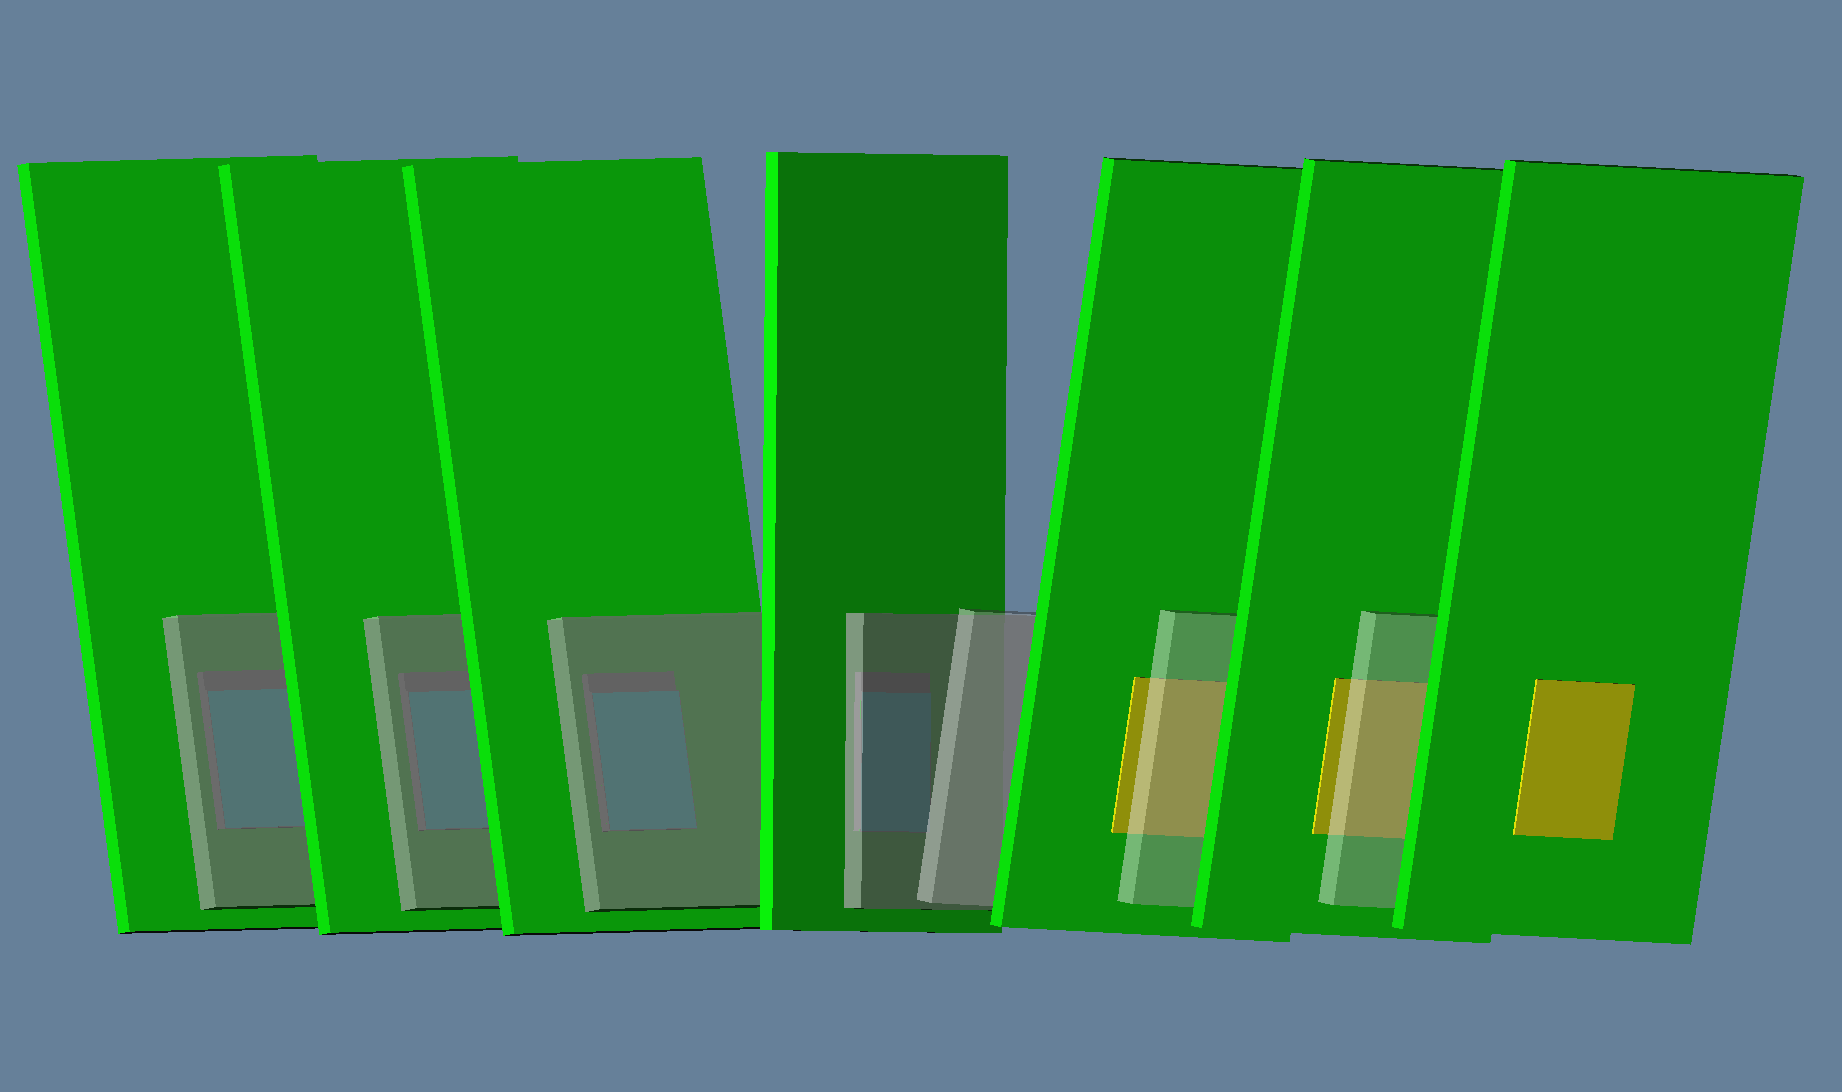
\includegraphics[width=\textwidth]{../figures/Telescope/AllpixTelescope.png}};

      \begin{scope}[x={(image.south east)},y={(image.north west)}]
        \node[above, color=white] at (0.5, 0.85) {The simulated
          Timepix3 telescope};
      \end{scope}
    \end{tikzpicture}
  \end{columns}

  \begin{itemize}
  \item \textcolor{Red}{Goal}:
    \begin{itemize}
    \item Simulate the test-beam setup.
    \item Extrapolate results for small-pitch pixels (e.g.  CLICpix
      with $25\,\micron$ pitch).
    \item Improve digitisation models for full-detector simulation.
    \end{itemize}
  \end{itemize}

\end{frame}

%%%%%%%%%%%%%%%%%%%%%%%%%%%%%
%         SLIDE             %
%%%%%%%%%%%%%%%%%%%%%%%%%%%%%
\begin{frame}
  \frametitle{The Timepix3 telescope performance}

  \begin{itemize}
  \item In simulation, extract the tracking resolution on the DUT
    using the Monte Carlo (MC) hit position
  \end{itemize}

  \begin{columns}
    \column{0.5\textwidth}
    \begin{itemize}
    \item Biased residual: reconstructed track vs. hit on the
      telescope planes.
    \item Agreement between data and simulation \ding{51}
    \end{itemize}

    \column{0.5\textwidth}
    \centering
    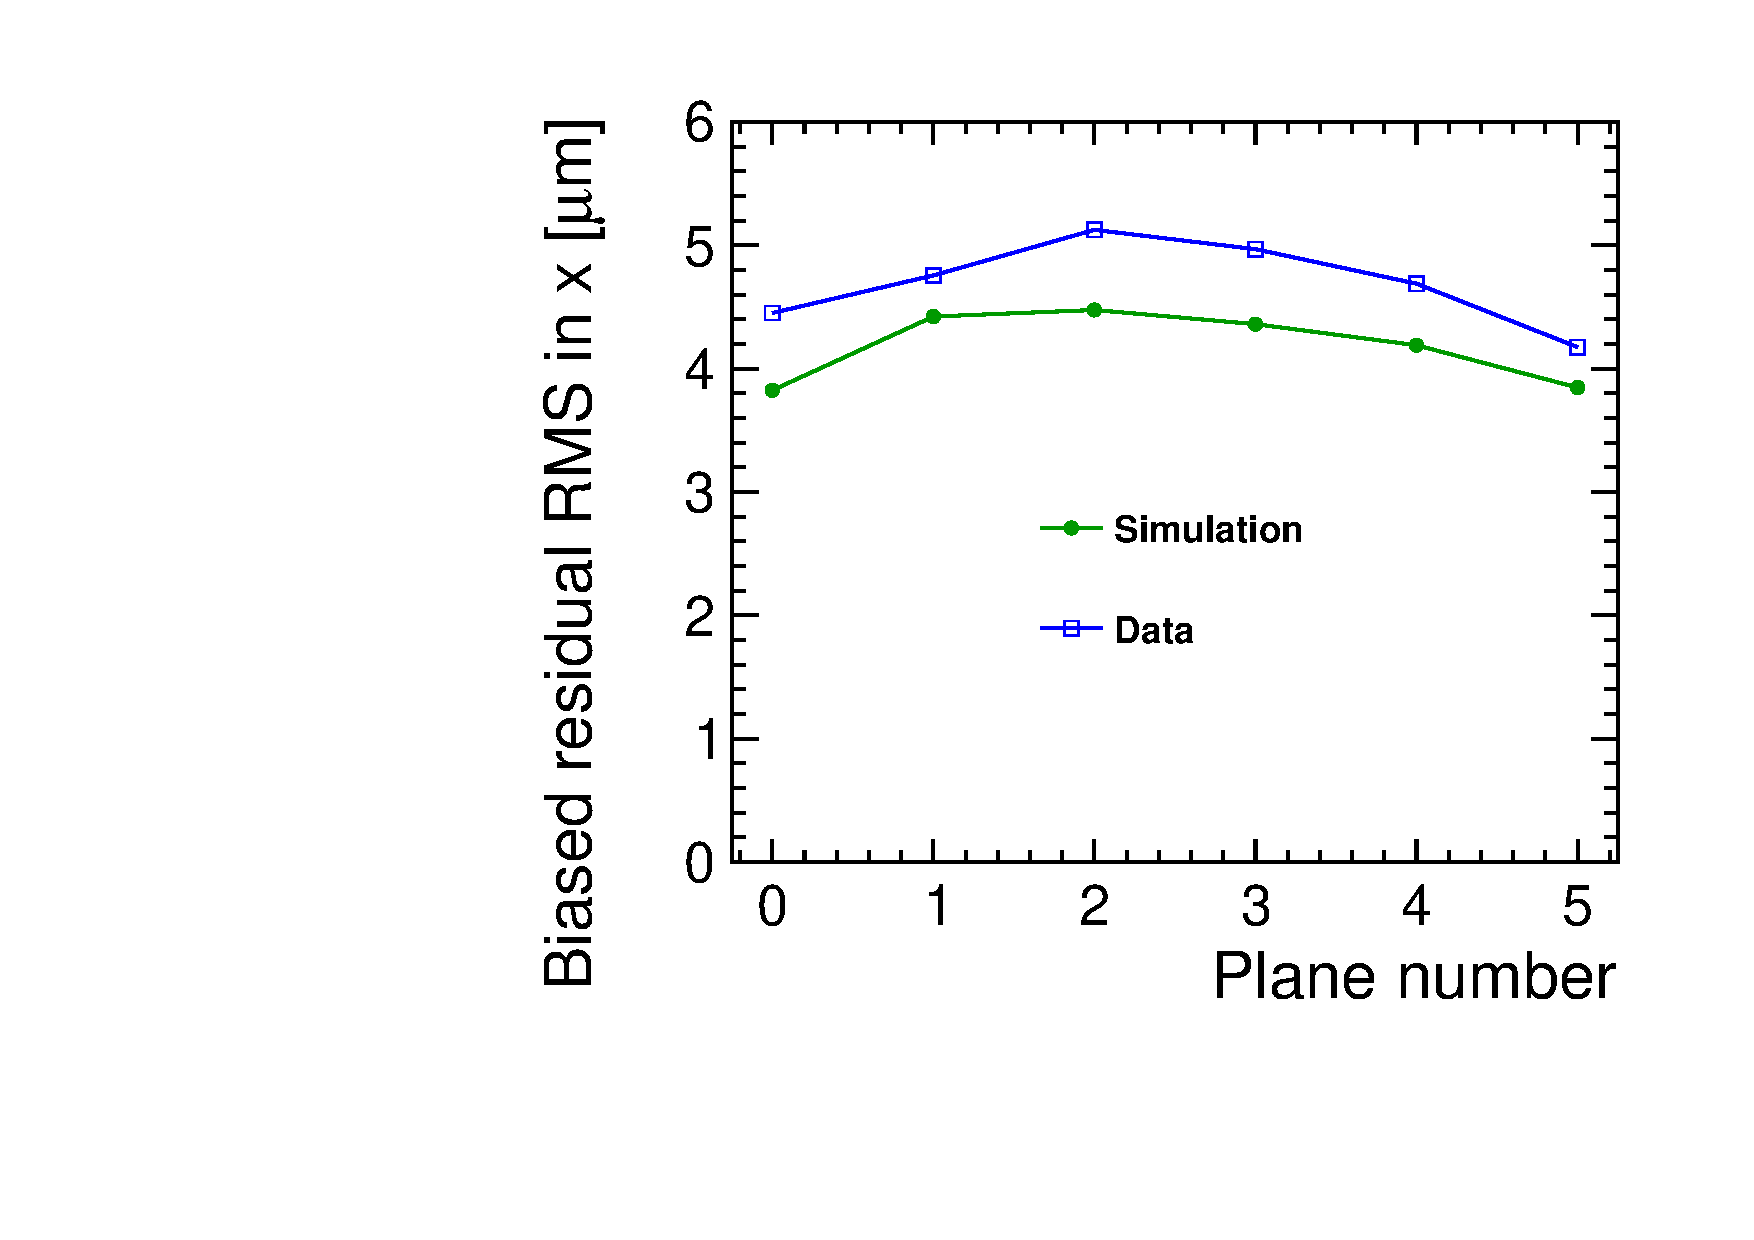
\includegraphics[width=0.8\textwidth]{../figures/Telescope/biasedResiduals/RMSX_simu_vs_data.pdf}
  \end{columns}

  \begin{columns}
    \column{0.5\textwidth}
    \begin{itemize}
    \item Tracking resolution on the DUT: reconstructed track vs. MC
      hit position
    \item Excellent tracking resolution of
      \textcolor{Green}{$\sim2\,\micron$} on the DUT
      \\
      $\Rightarrow$ In agreement with the expectations \ding{51}
    \end{itemize}

    \column{0.5\textwidth}
    \centering
    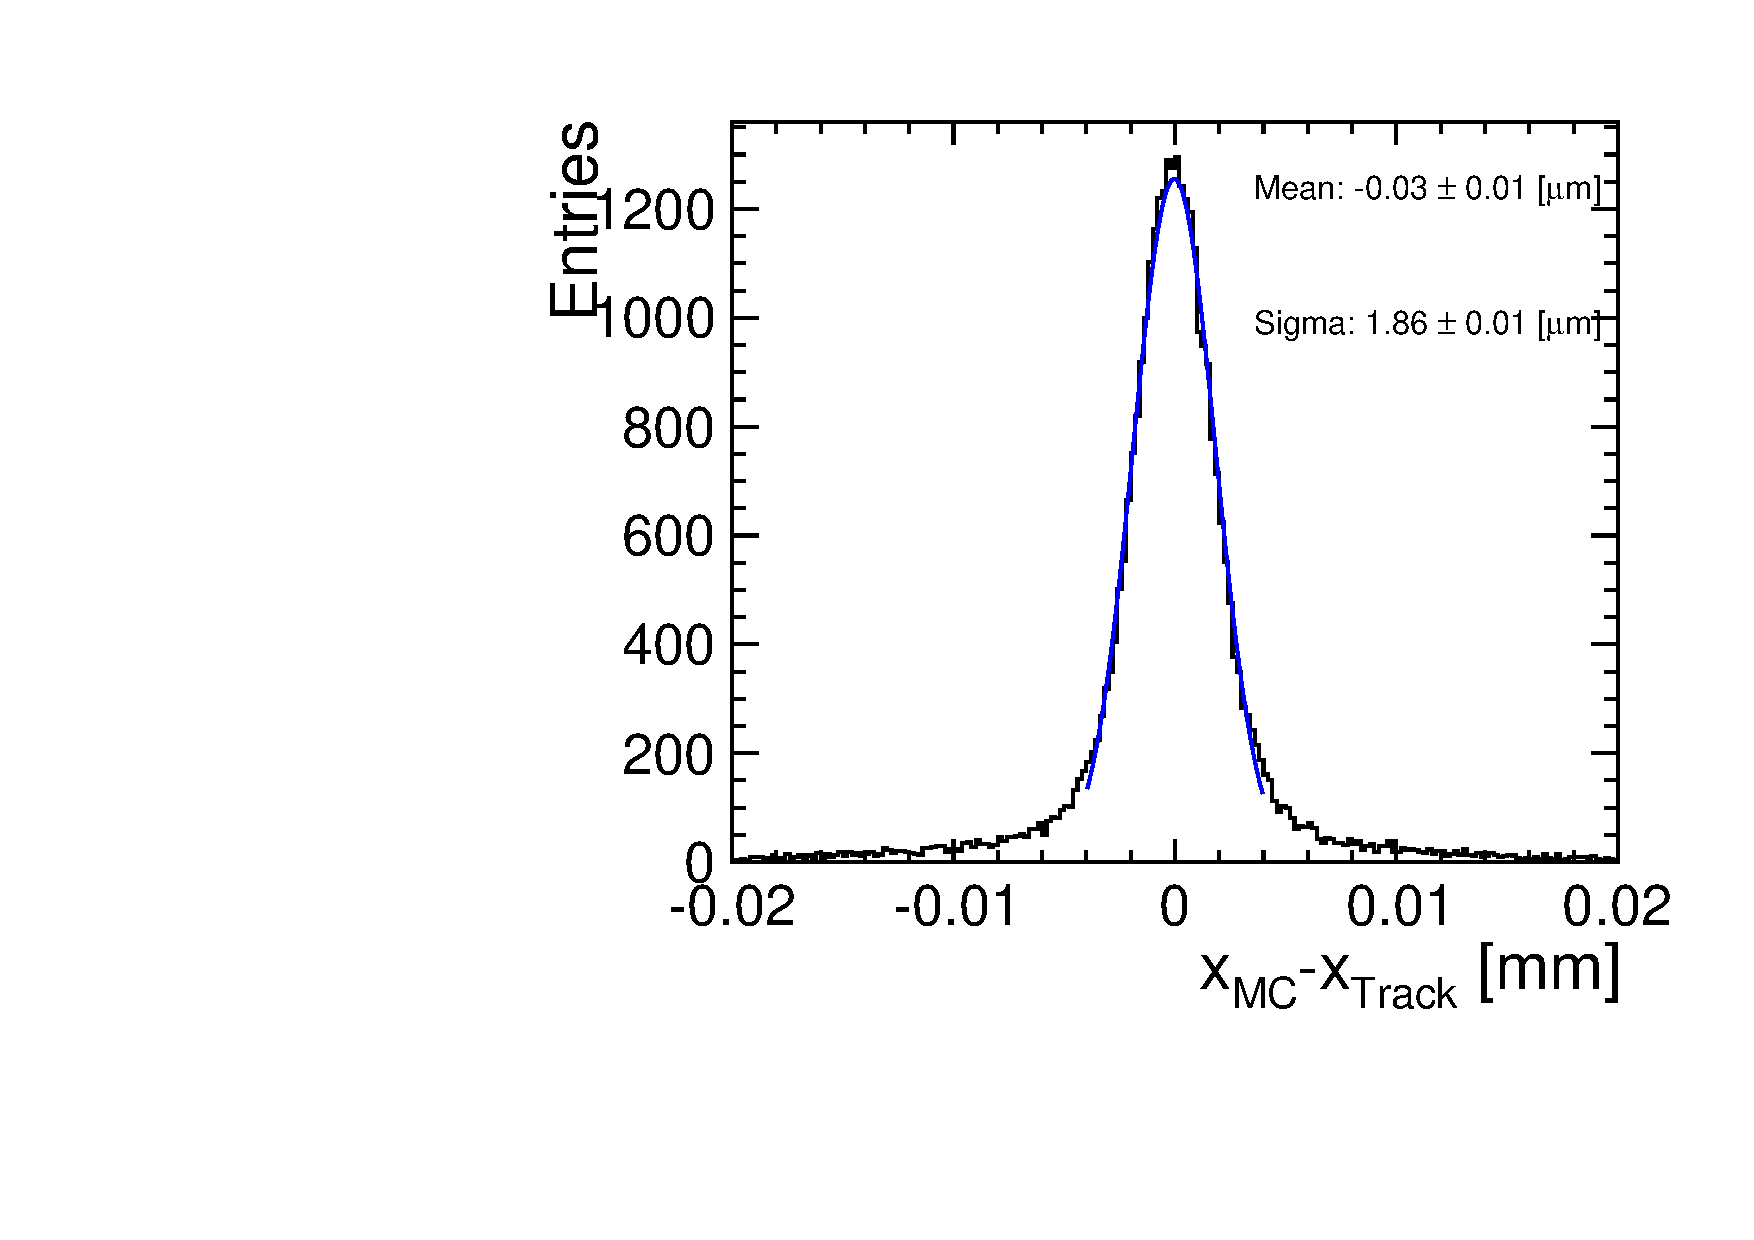
\includegraphics[width=0.8\textwidth]{../figures/Telescope/Unbiased_trackRes_DUT_x.pdf}
  \end{columns}

\end{frame}

%%%%%%%%%%%%%%%%%%%%%%%%%%%%%
%         SLIDE             %
%%%%%%%%%%%%%%%%%%%%%%%%%%%%%
\begin{frame}
  \frametitle{Thin sensors studies}

  \begin{itemize}
  \item Prototypes with Advacam planar n-in-p thin sensors
    ($50 - 150\,\micron$ thick) bump-bonded to Timepix3 readout ASICs
  \item Tested in test-beam measurements and compared with AllPix
    simulations
  \end{itemize}

\end{frame}

%%%%%%%%%%%%%%%%%%%%%%%%%%%%%
%         SLIDE             %
%%%%%%%%%%%%%%%%%%%%%%%%%%%%%
\begin{frame}
  \frametitle{Validation of the energy deposition}

  \begin{itemize}
  \item Validation of the calibration
  \item Validation of the \textsc{Geant4} simulation: PAI physics list
    (Bichsel model).
  \end{itemize}

  \begin{columns}
    \column{0.3\textwidth}
    \begin{itemize}
    \item $50\,\micron$
    \end{itemize}
    \centering
    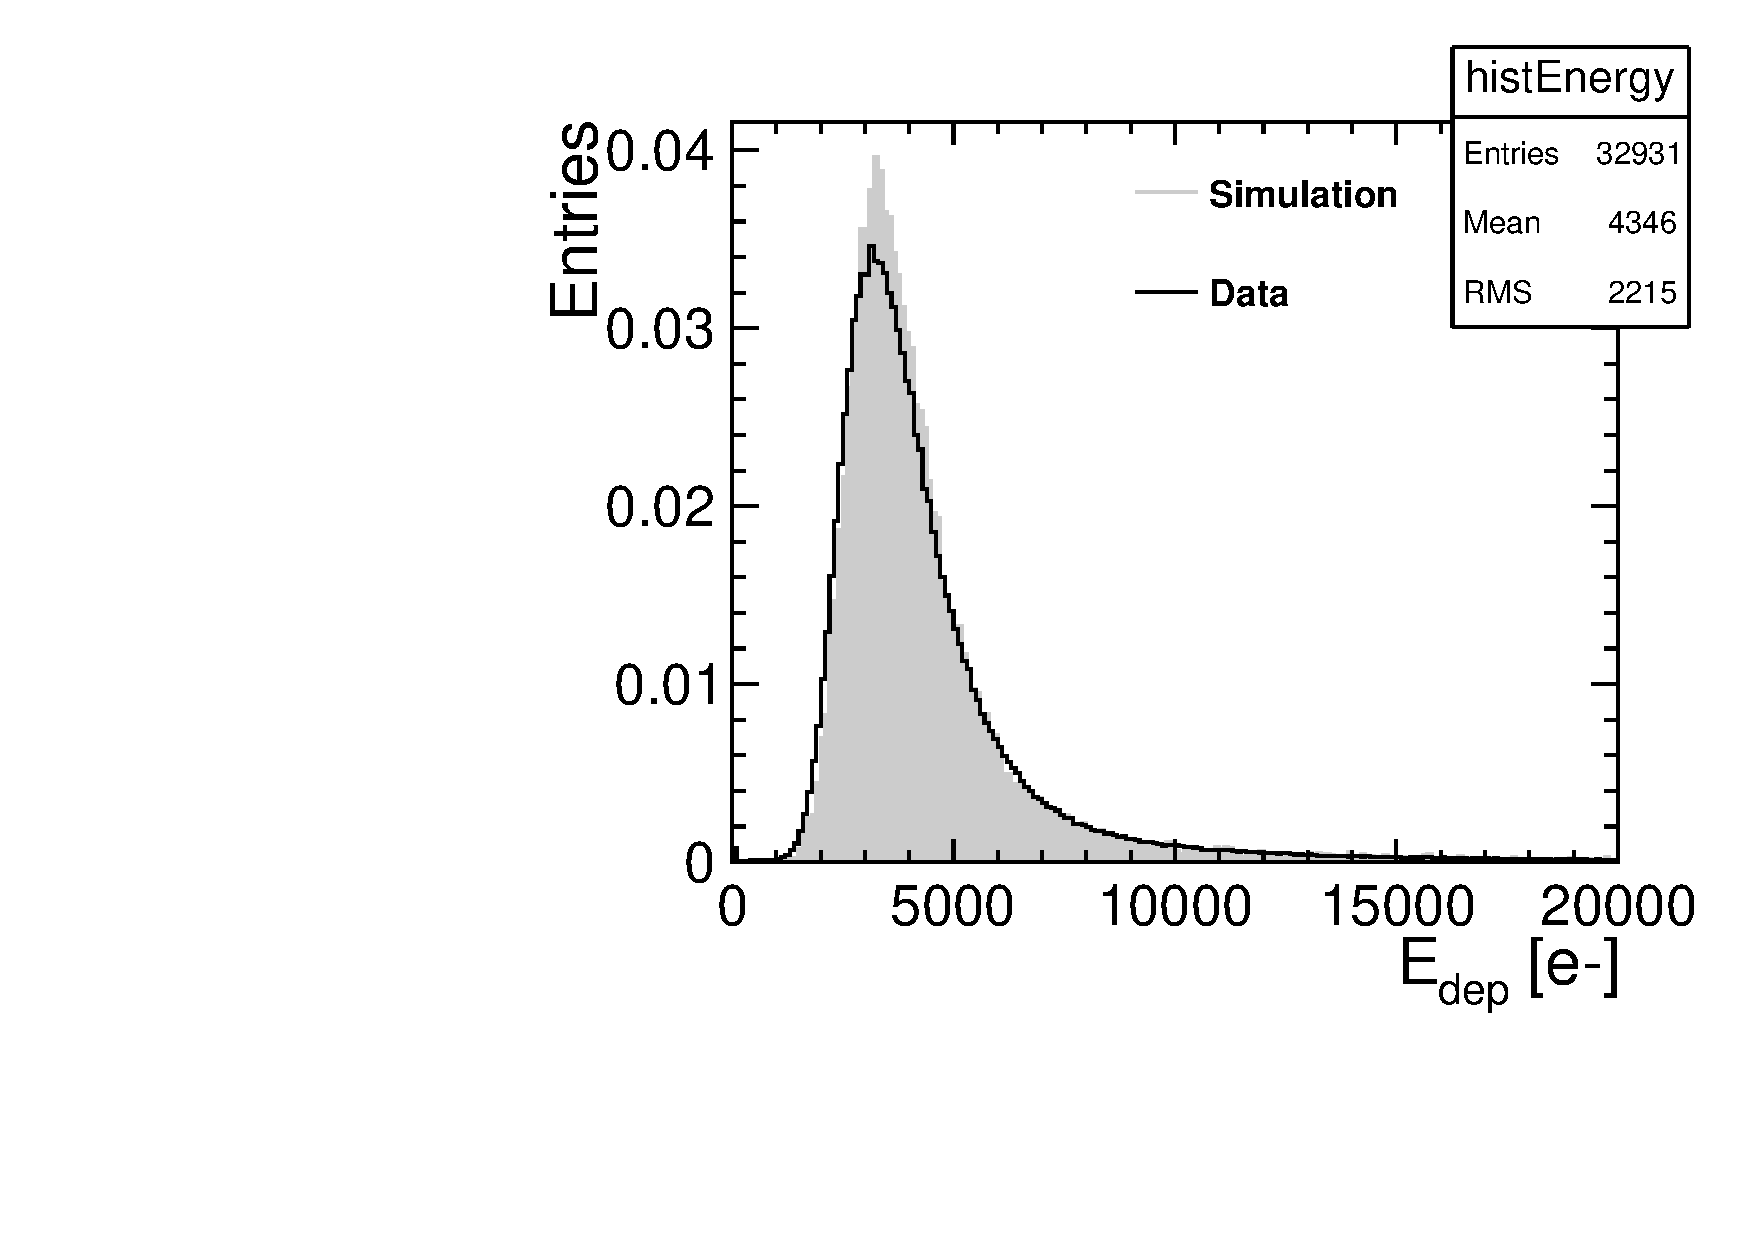
\includegraphics[width=\textwidth]{../figures/TestBeam/50micron_Edep.pdf}

    \column{0.3\textwidth}
    \begin{itemize}
    \item $100\,\micron$
    \end{itemize}
    \centering
    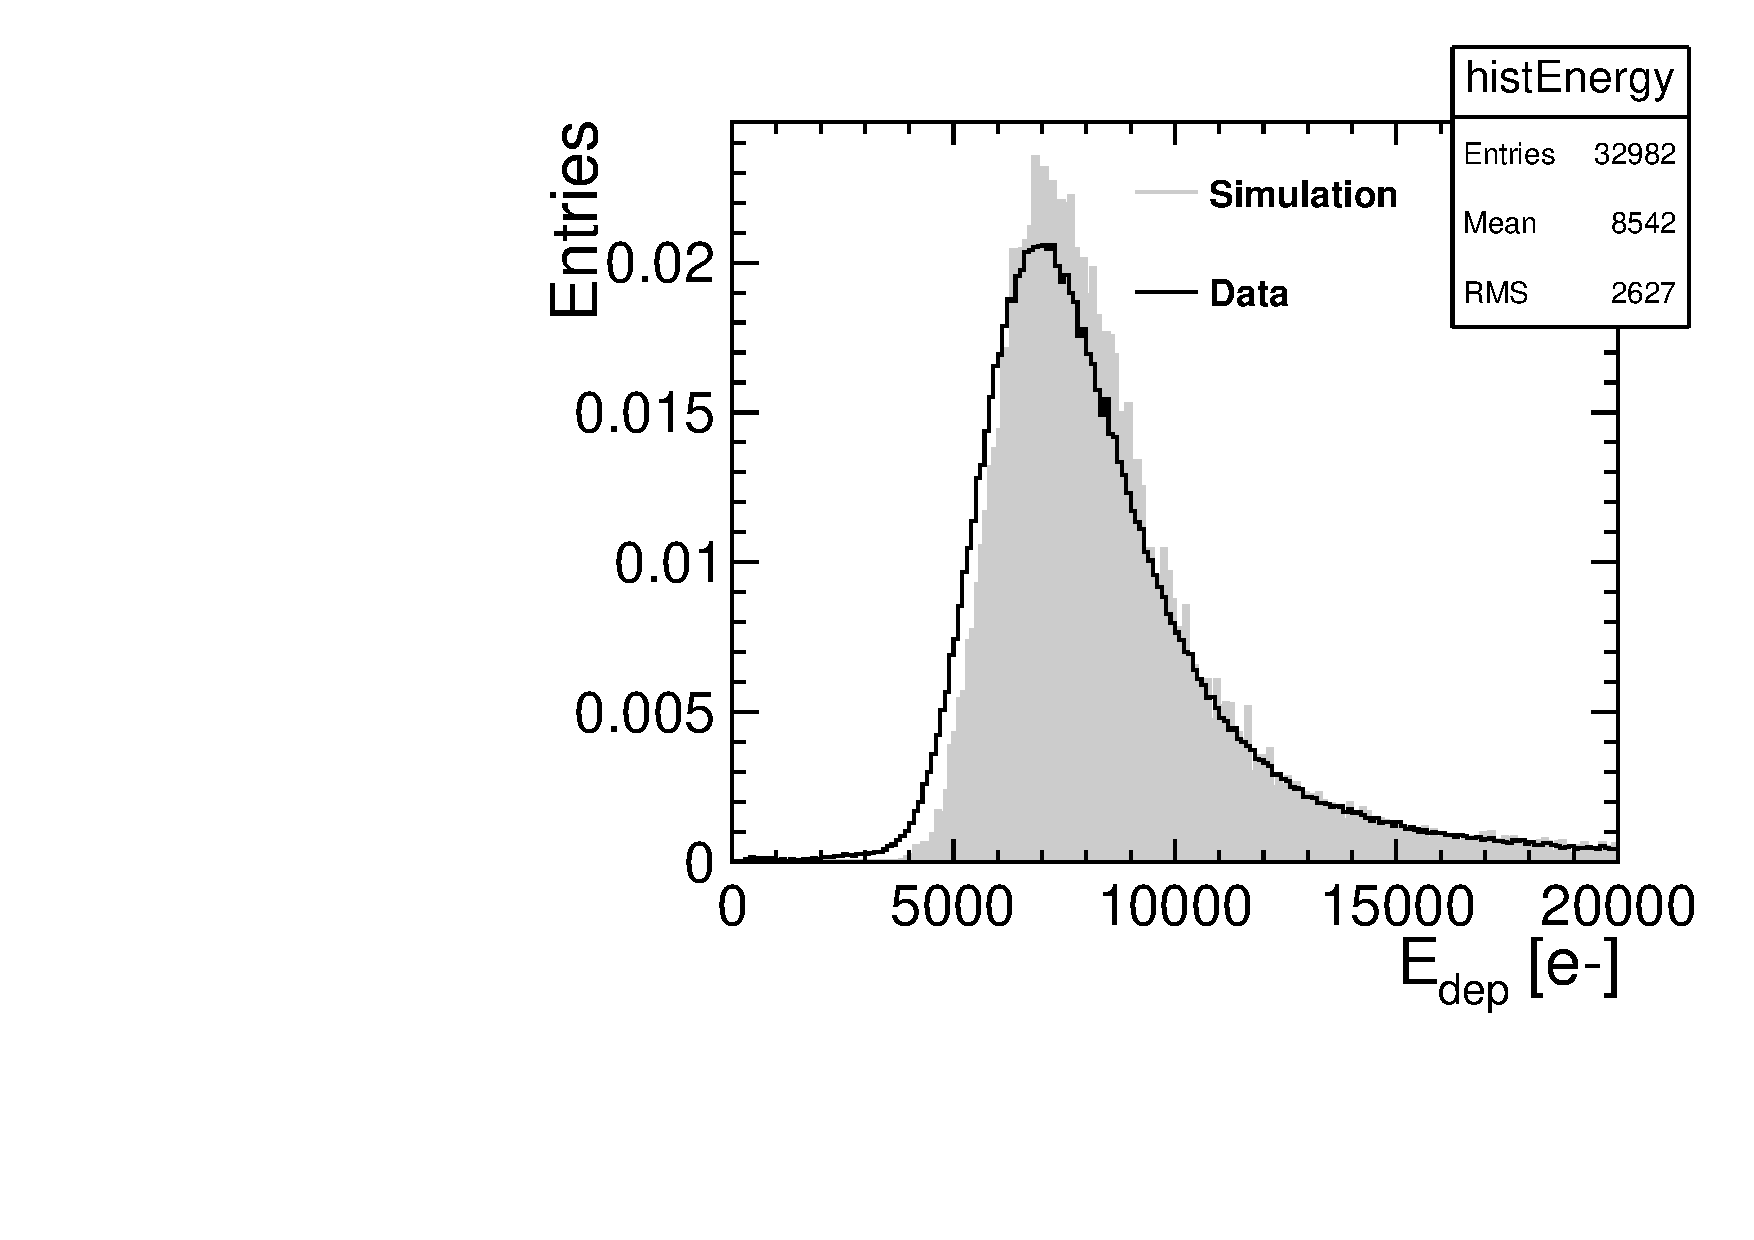
\includegraphics[width=\textwidth]{../figures/TestBeam/100micron_Edep.pdf}

    \column{0.3\textwidth}
    \begin{itemize}
    \item $150\,\micron$
    \end{itemize}
    \centering
    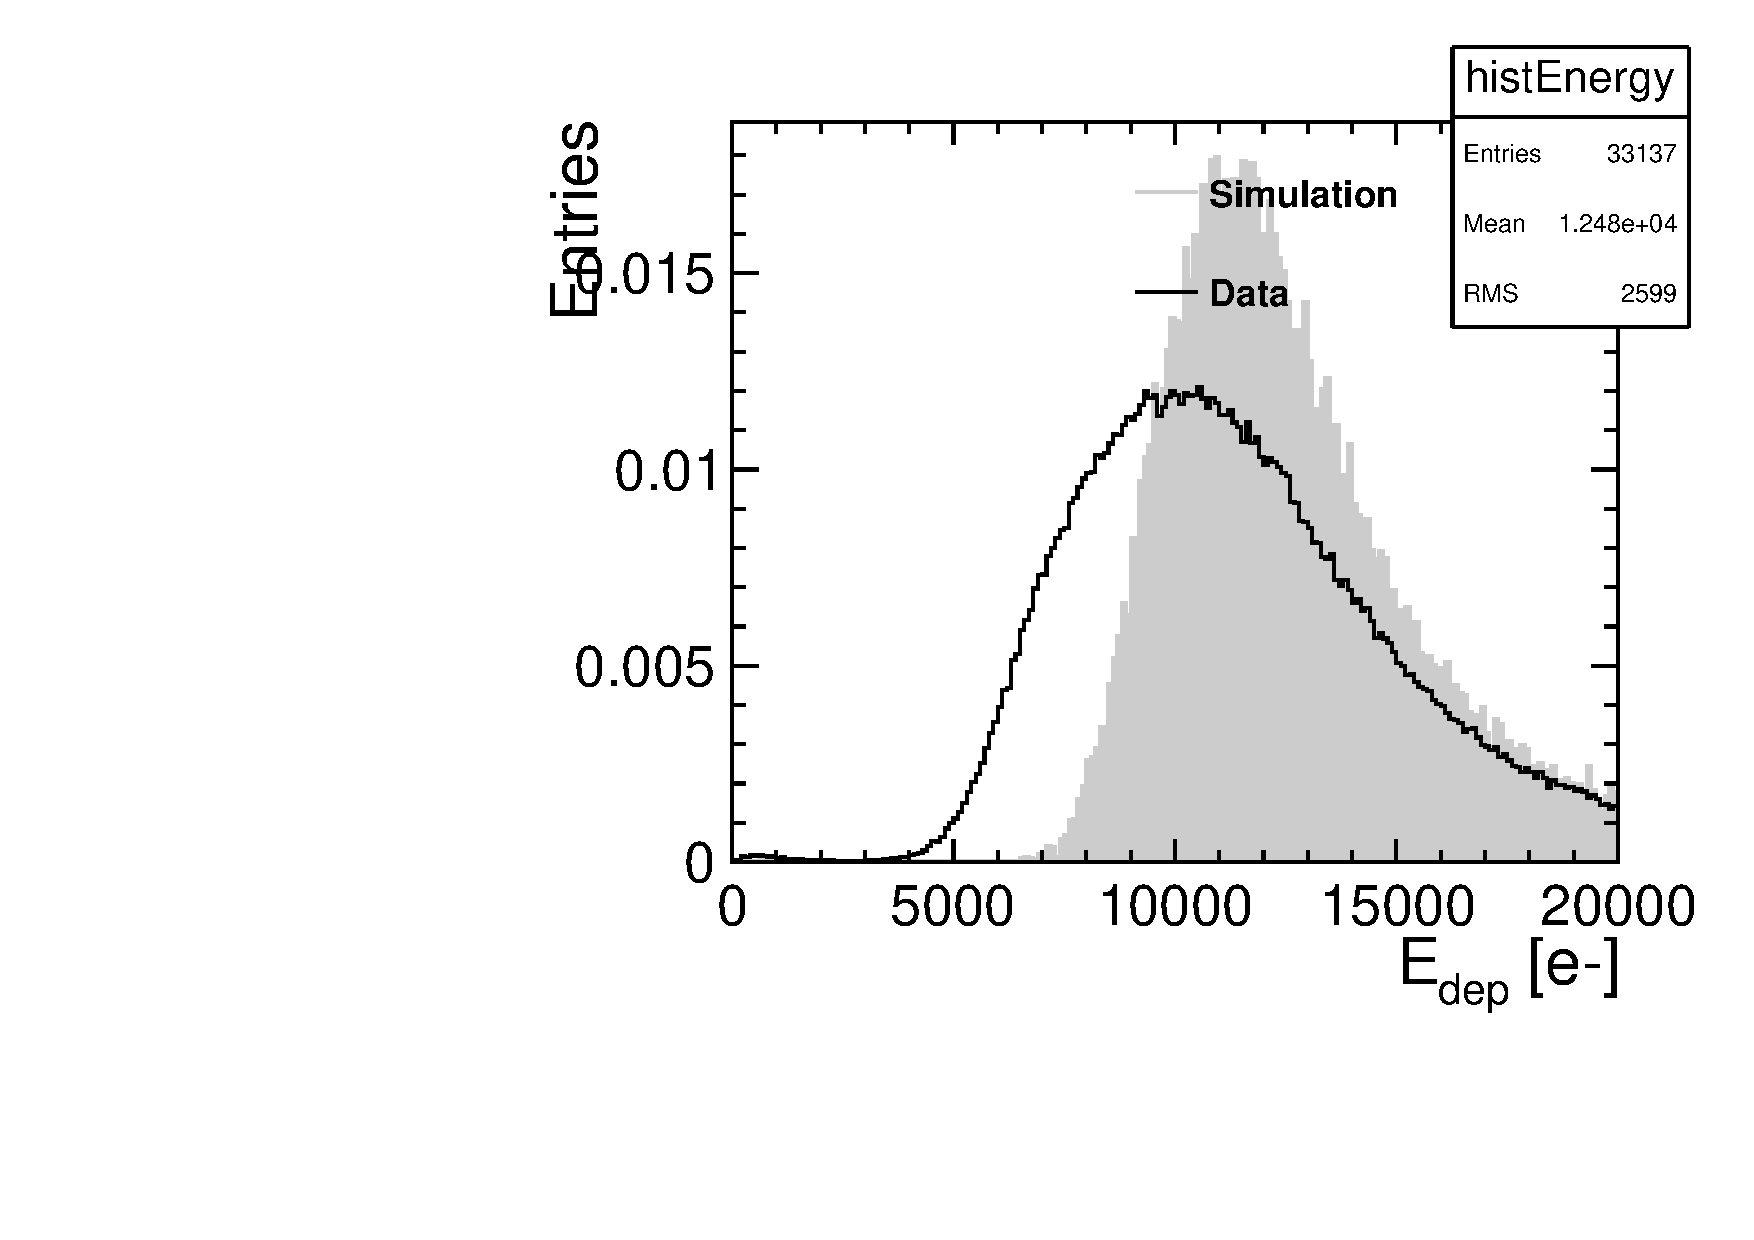
\includegraphics[width=\textwidth]{../figures/TestBeam/150micron_Edep.pdf}
  \end{columns}

\end{frame}

%%%%%%%%%%%%%%%%%%%%%%%%%%%%%
%         SLIDE             %
%%%%%%%%%%%%%%%%%%%%%%%%%%%%%
\begin{frame}
  \frametitle{Charge sharing}

  \begin{columns}[t]
    \column{0.25\textwidth}
    \begin{itemize}
    \item 1-pixel cluster
    \end{itemize}
    \begin{tikzpicture}
      \draw (0,0) rectangle (0.5,-0.5);
    \end{tikzpicture}
    \centering
    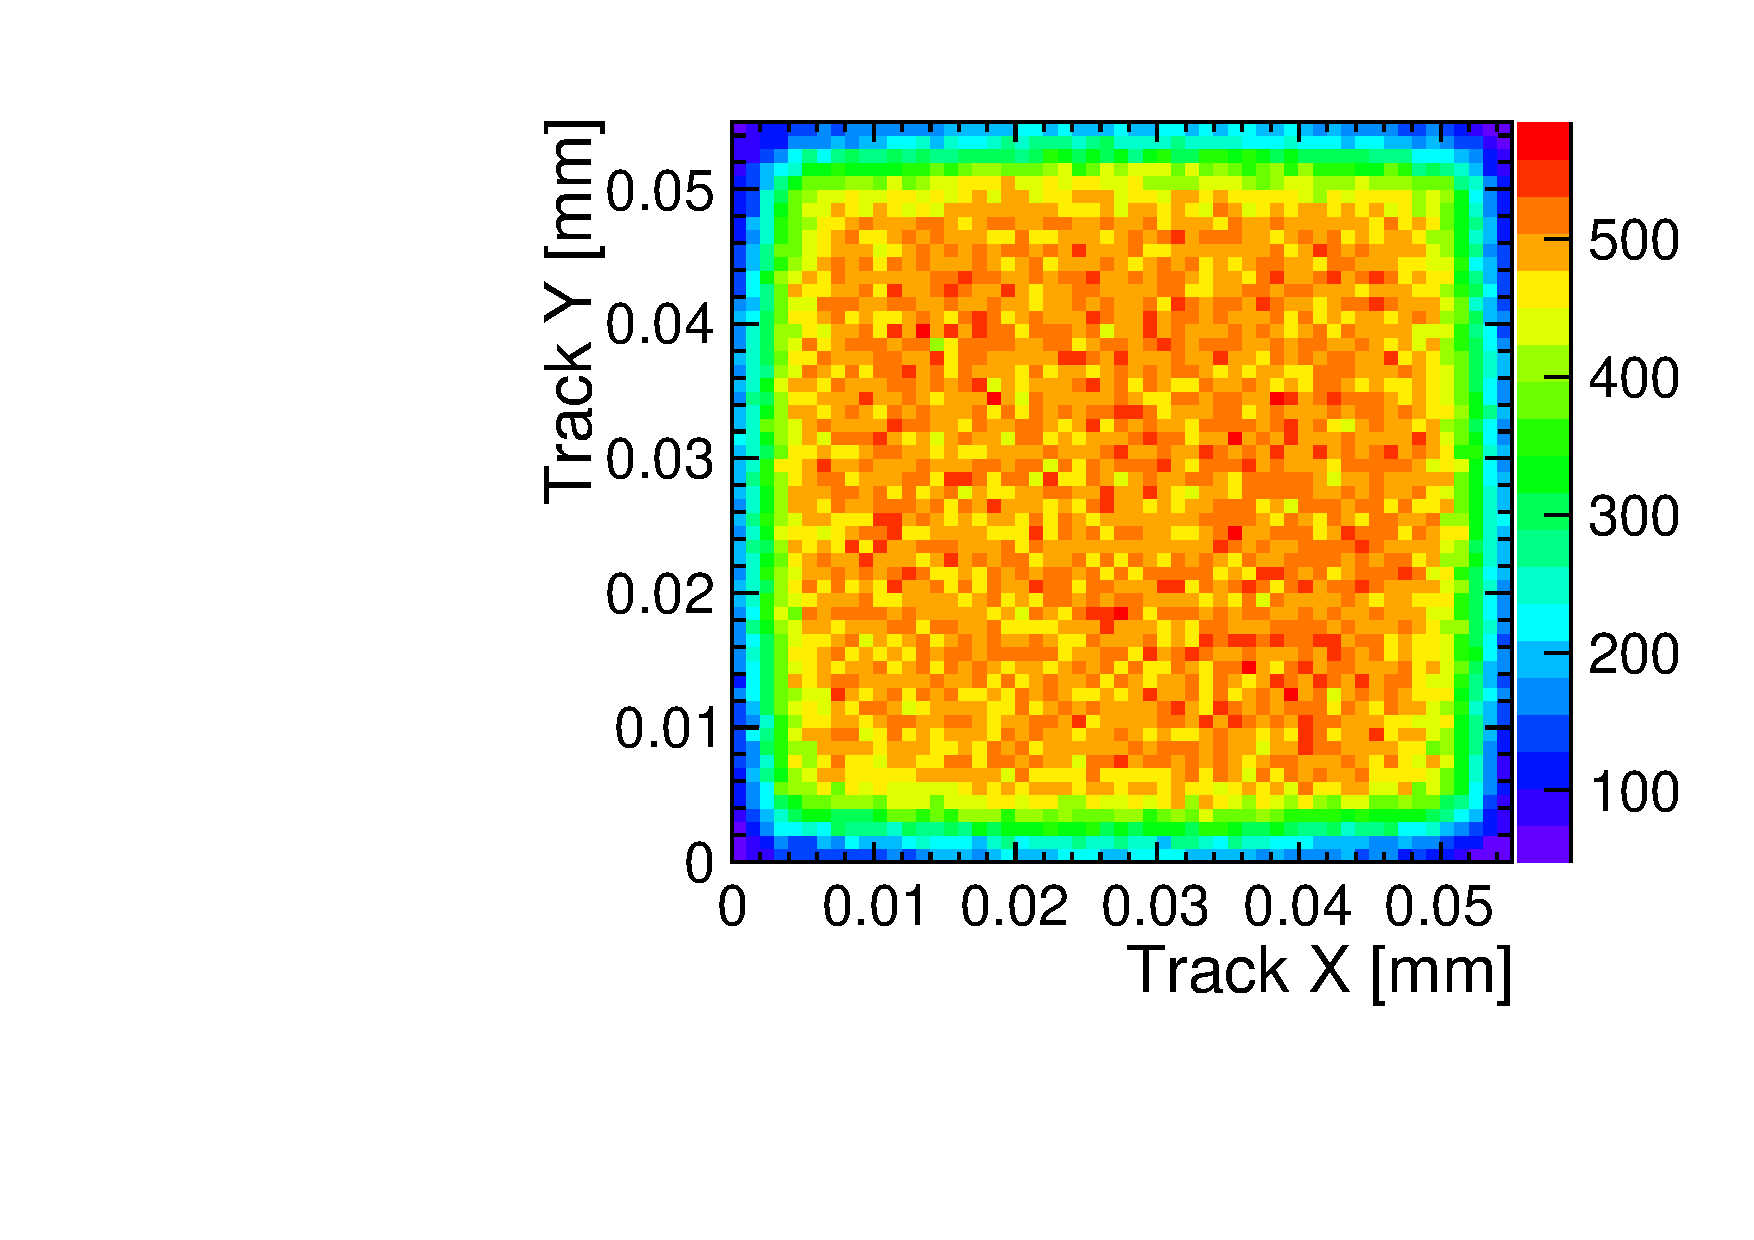
\includegraphics[width=\textwidth]{../figures/TestBeam/TrackPosWPixel_1hit_runW19_G7.pdf}

    \column{0.25\textwidth}
    \begin{itemize}
    \item 2-pixel cluster
    \end{itemize}
    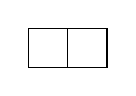
\begin{tikzpicture}
      \draw (0.0,0.0) rectangle (0.5,-0.5);
      \draw (0.5,0.0) rectangle (1.0,-0.5);
    \end{tikzpicture}
    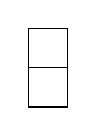
\begin{tikzpicture}
      \draw (0.0,0.0) rectangle (0.5,-0.5);
      \draw (0.0,0.5) rectangle (0.5,0.0);
    \end{tikzpicture}
    \centering
    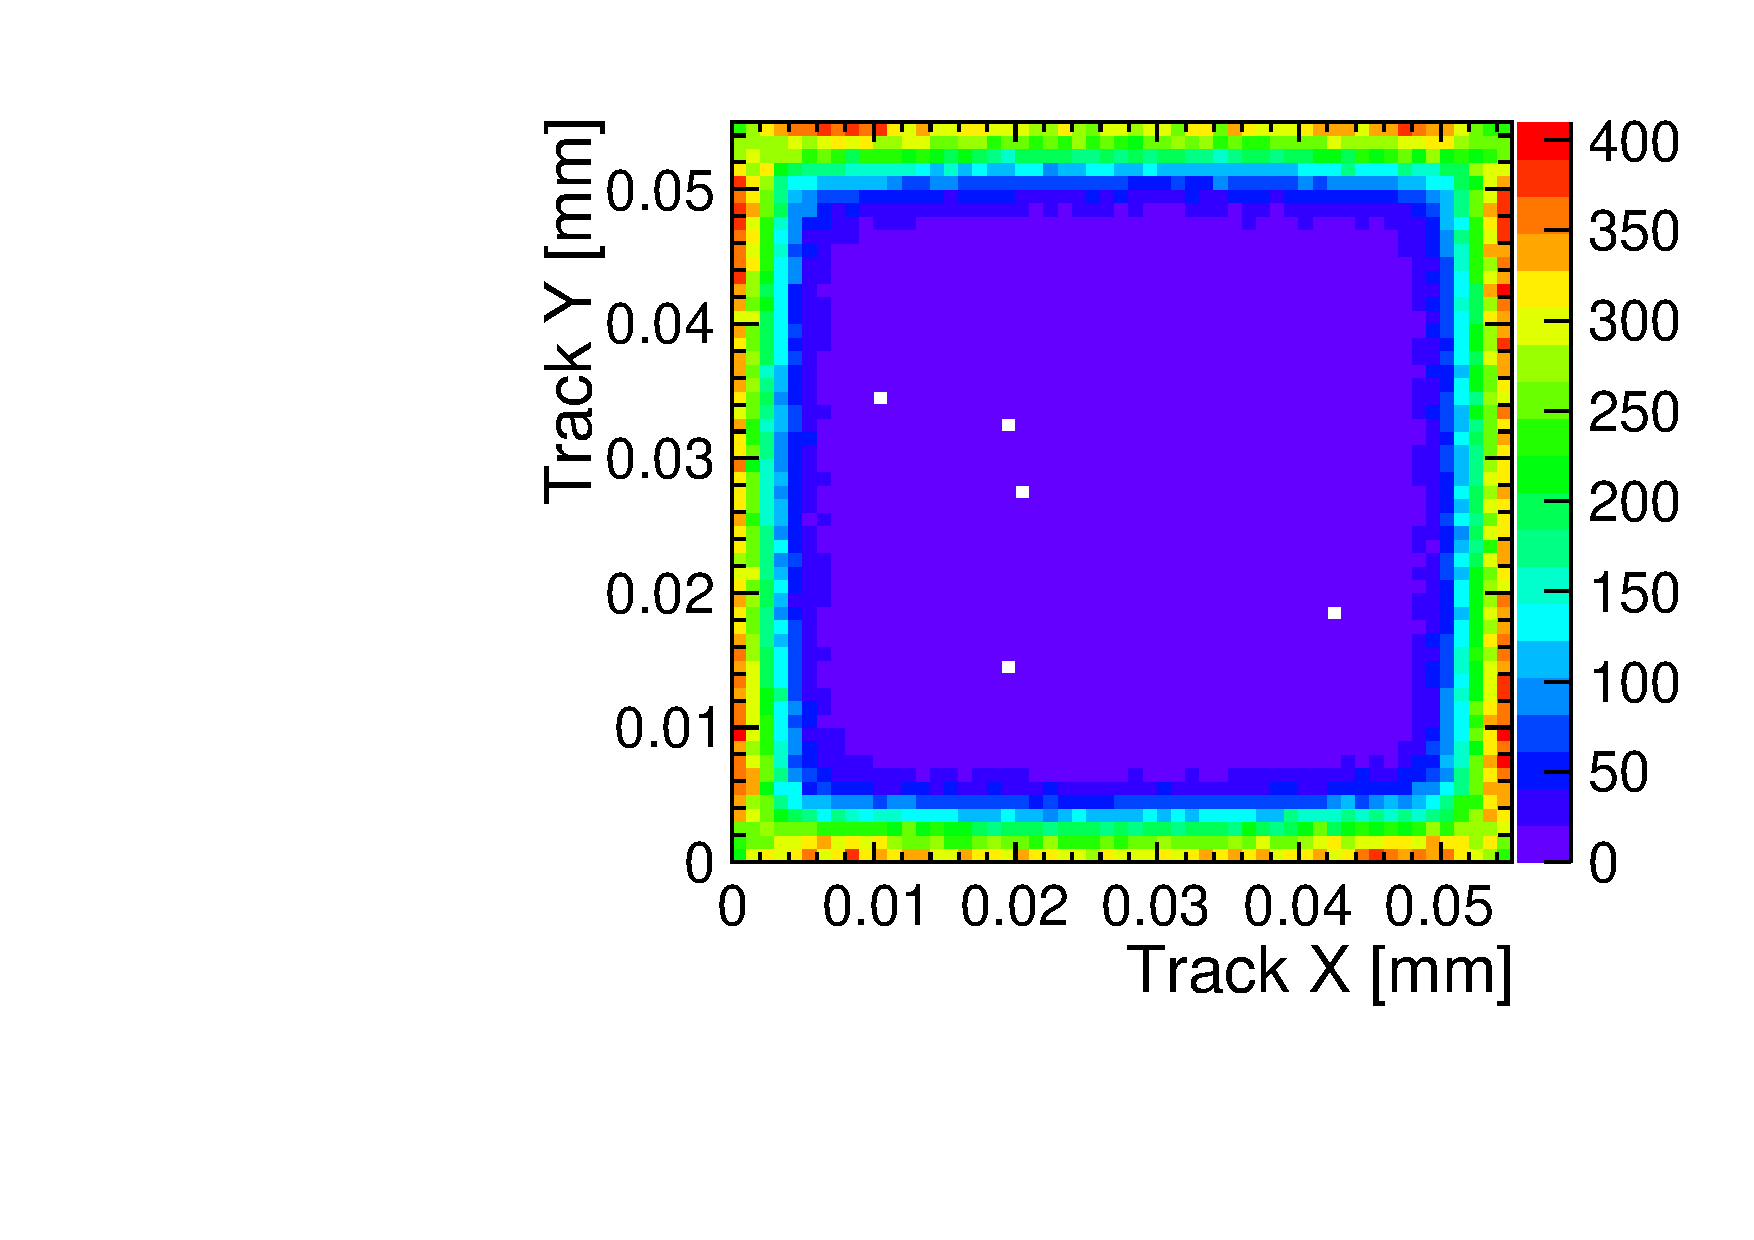
\includegraphics[width=\textwidth]{../figures/TestBeam/TrackPosWPixel_2hit_runW19_G7.pdf}

    \column{0.25\textwidth}
    \begin{itemize}
    \item 3-pixel cluster
    \end{itemize}
    
\begin{tikzpicture}
      \draw (0.0,0.0) rectangle (0.5,-0.5);
      \draw (0.5,-0.5) rectangle (1.0,-1.0);
      \draw (0.5,0.0) rectangle (1.0,-0.5);
    \end{tikzpicture}
    \centering
    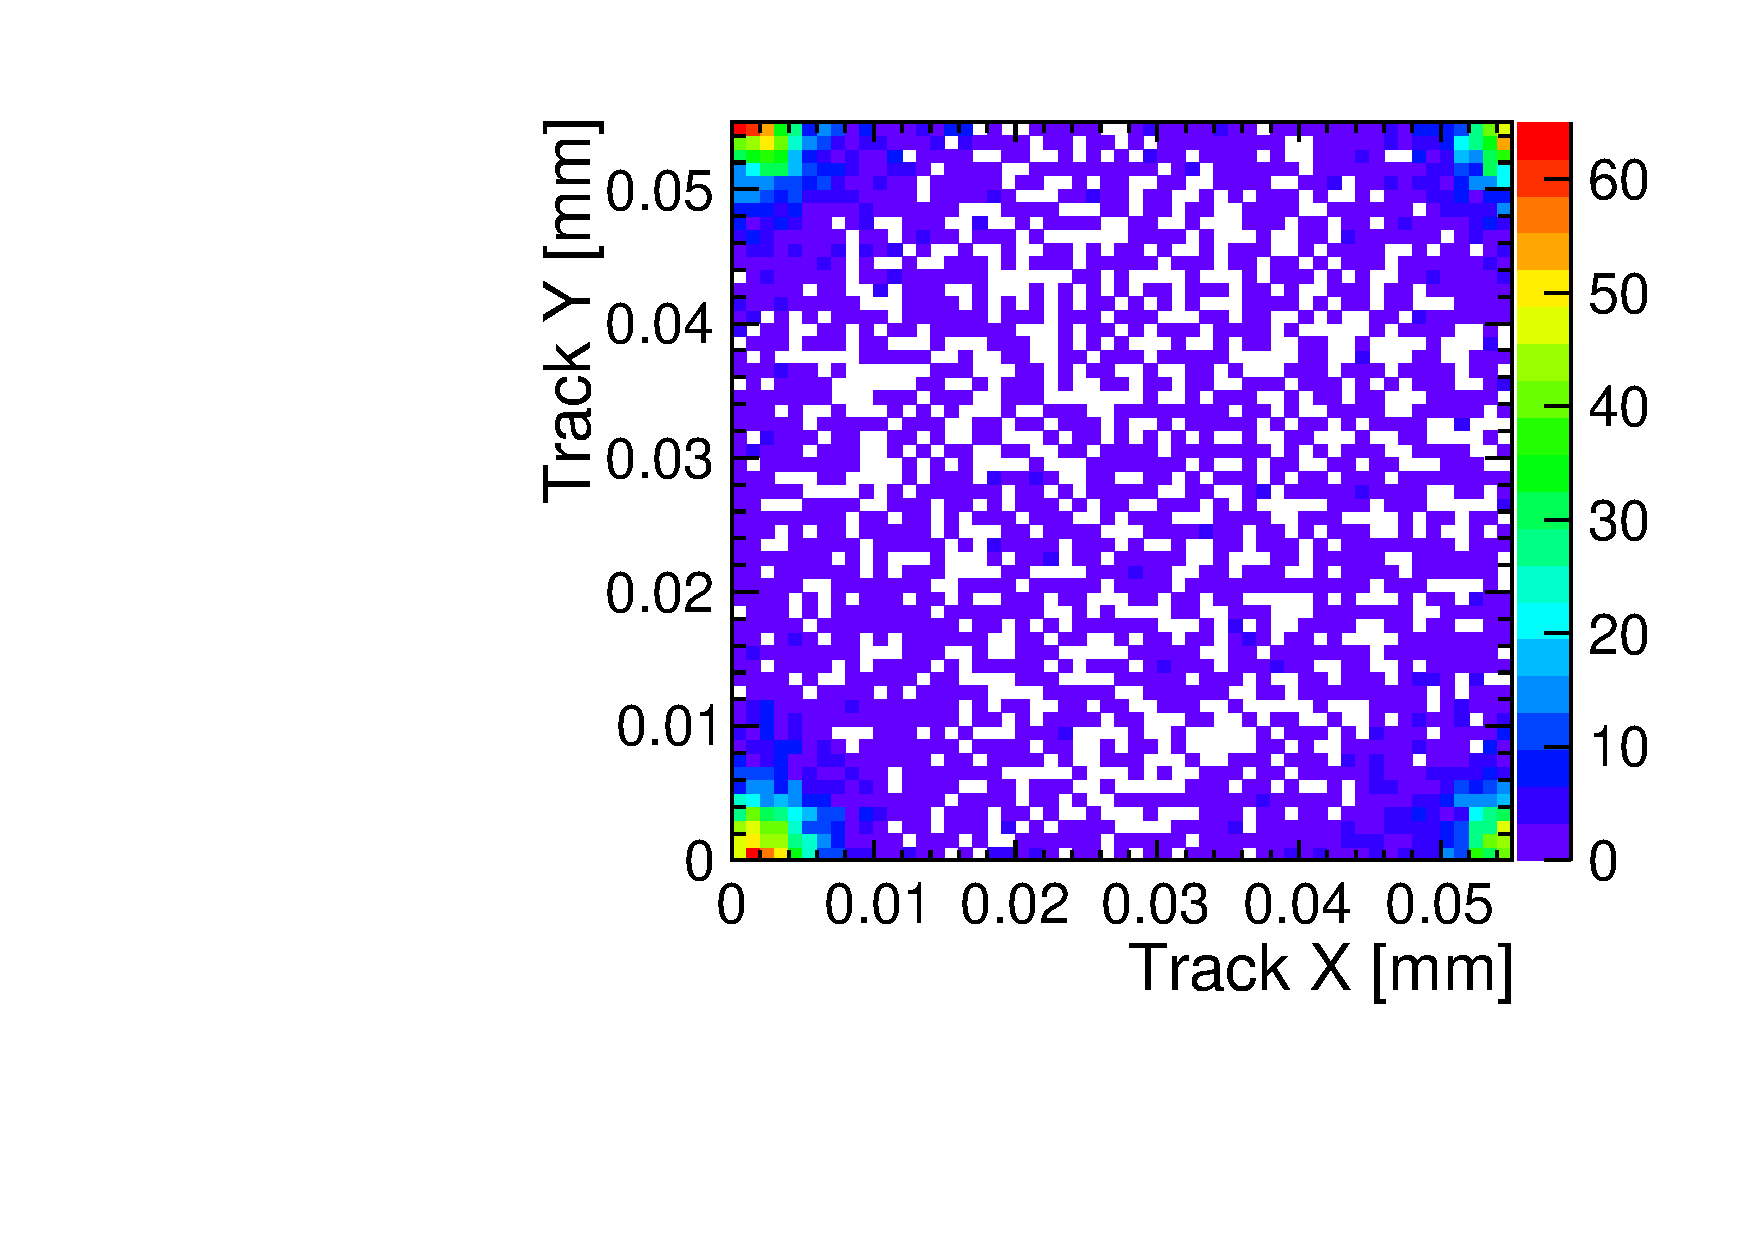
\includegraphics[width=\textwidth]{../figures/TestBeam/TrackPosWPixel_3hit_runW19_G7.pdf}

    \column{0.25\textwidth}
    \begin{itemize}
    \item 4-pixel cluster
    \end{itemize}
    
\begin{tikzpicture}
      \draw (0.0,0.0) rectangle (0.5,-0.5);
      \draw (0.5,-0.5) rectangle (1.0,-1.0);
      \draw (0.5,0.0) rectangle (1.0,-0.5);
      \draw (0.0,-0.5) rectangle (0.5,-1.0);
    \end{tikzpicture}
    \centering
    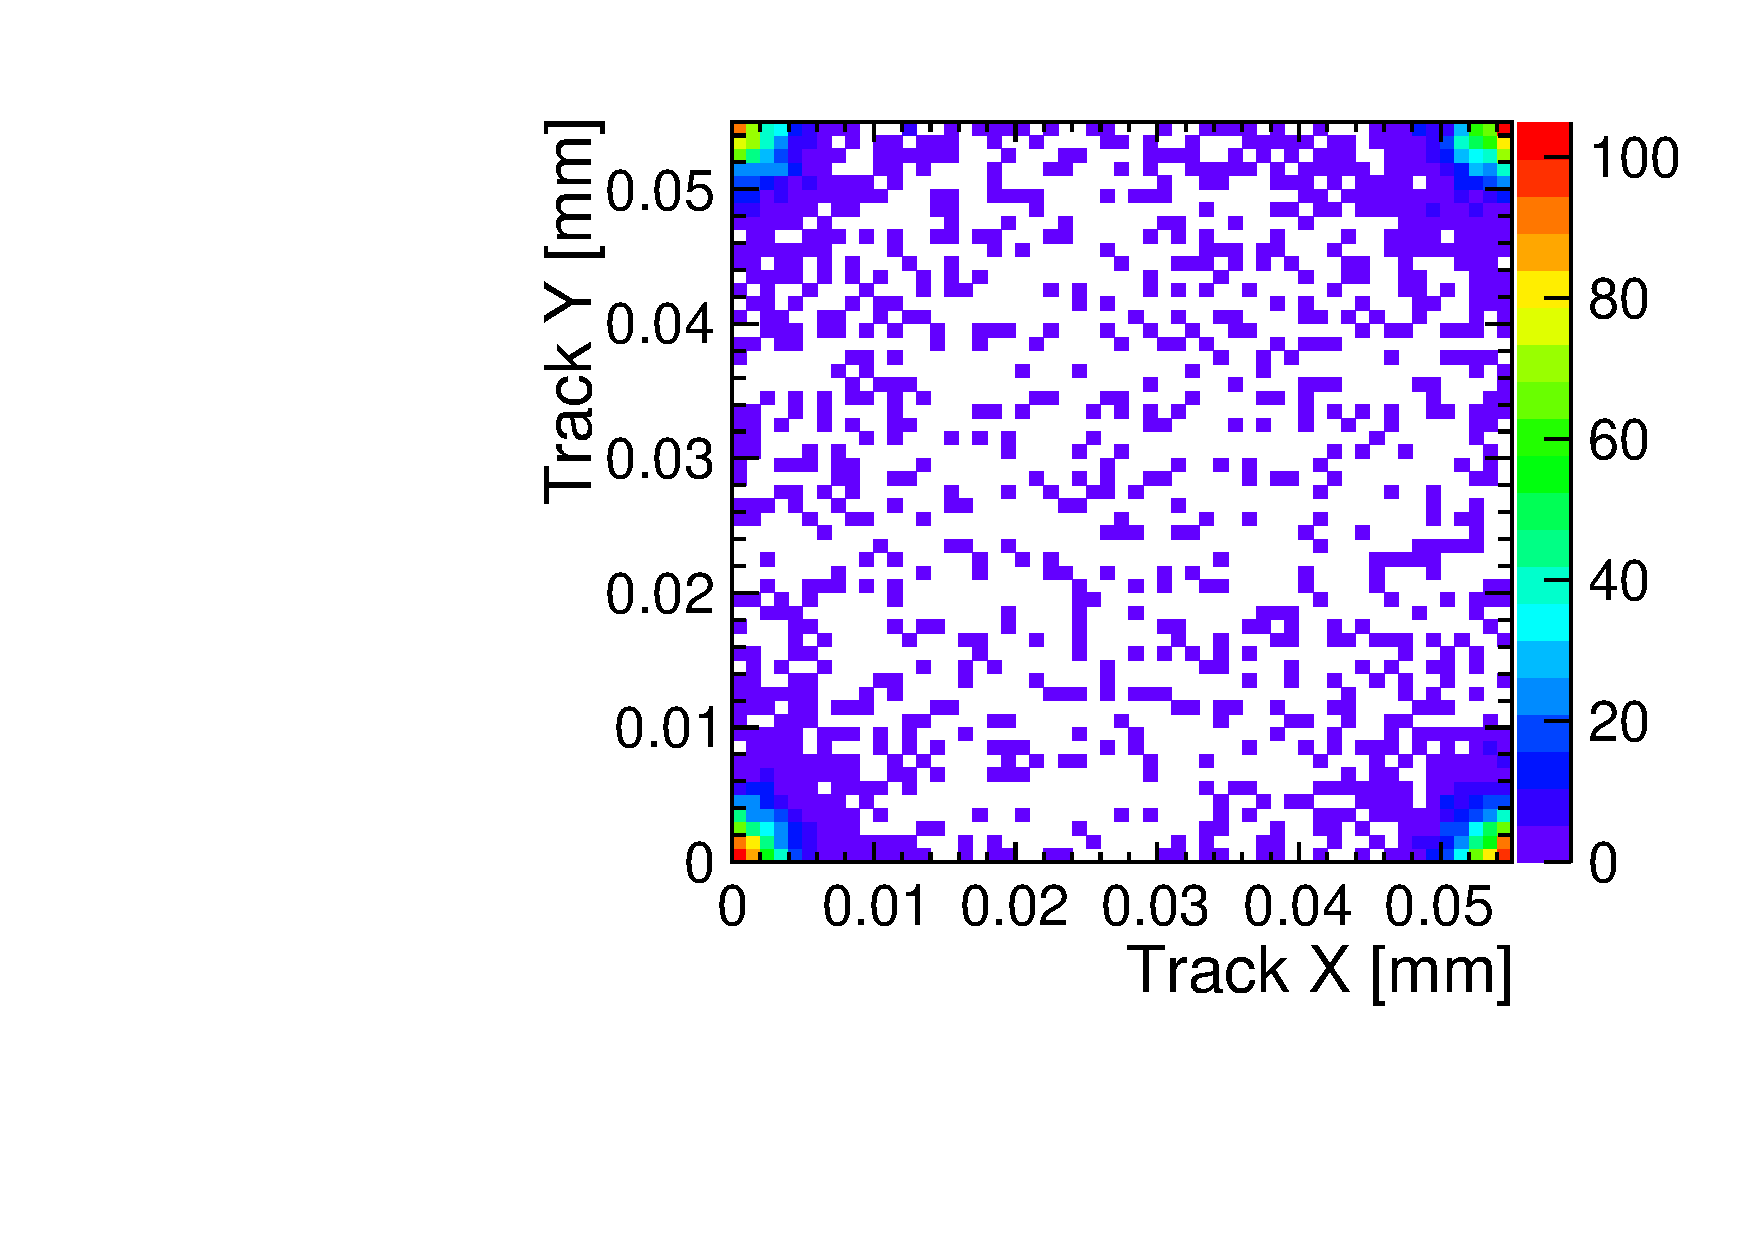
\includegraphics[width=\textwidth]{../figures/TestBeam/TrackPosWPixel_4hit_runW19_G7.pdf}
  \end{columns}

\end{frame}

%%%%%%%%%%%%%%%%%%%%%%%%%%%%%
%         SLIDE             %
%%%%%%%%%%%%%%%%%%%%%%%%%%%%%
\begin{frame}
  \frametitle{Cluster-sizes \& resolution}

  \begin{columns}
    \column{0.5\textwidth}
    \centering
    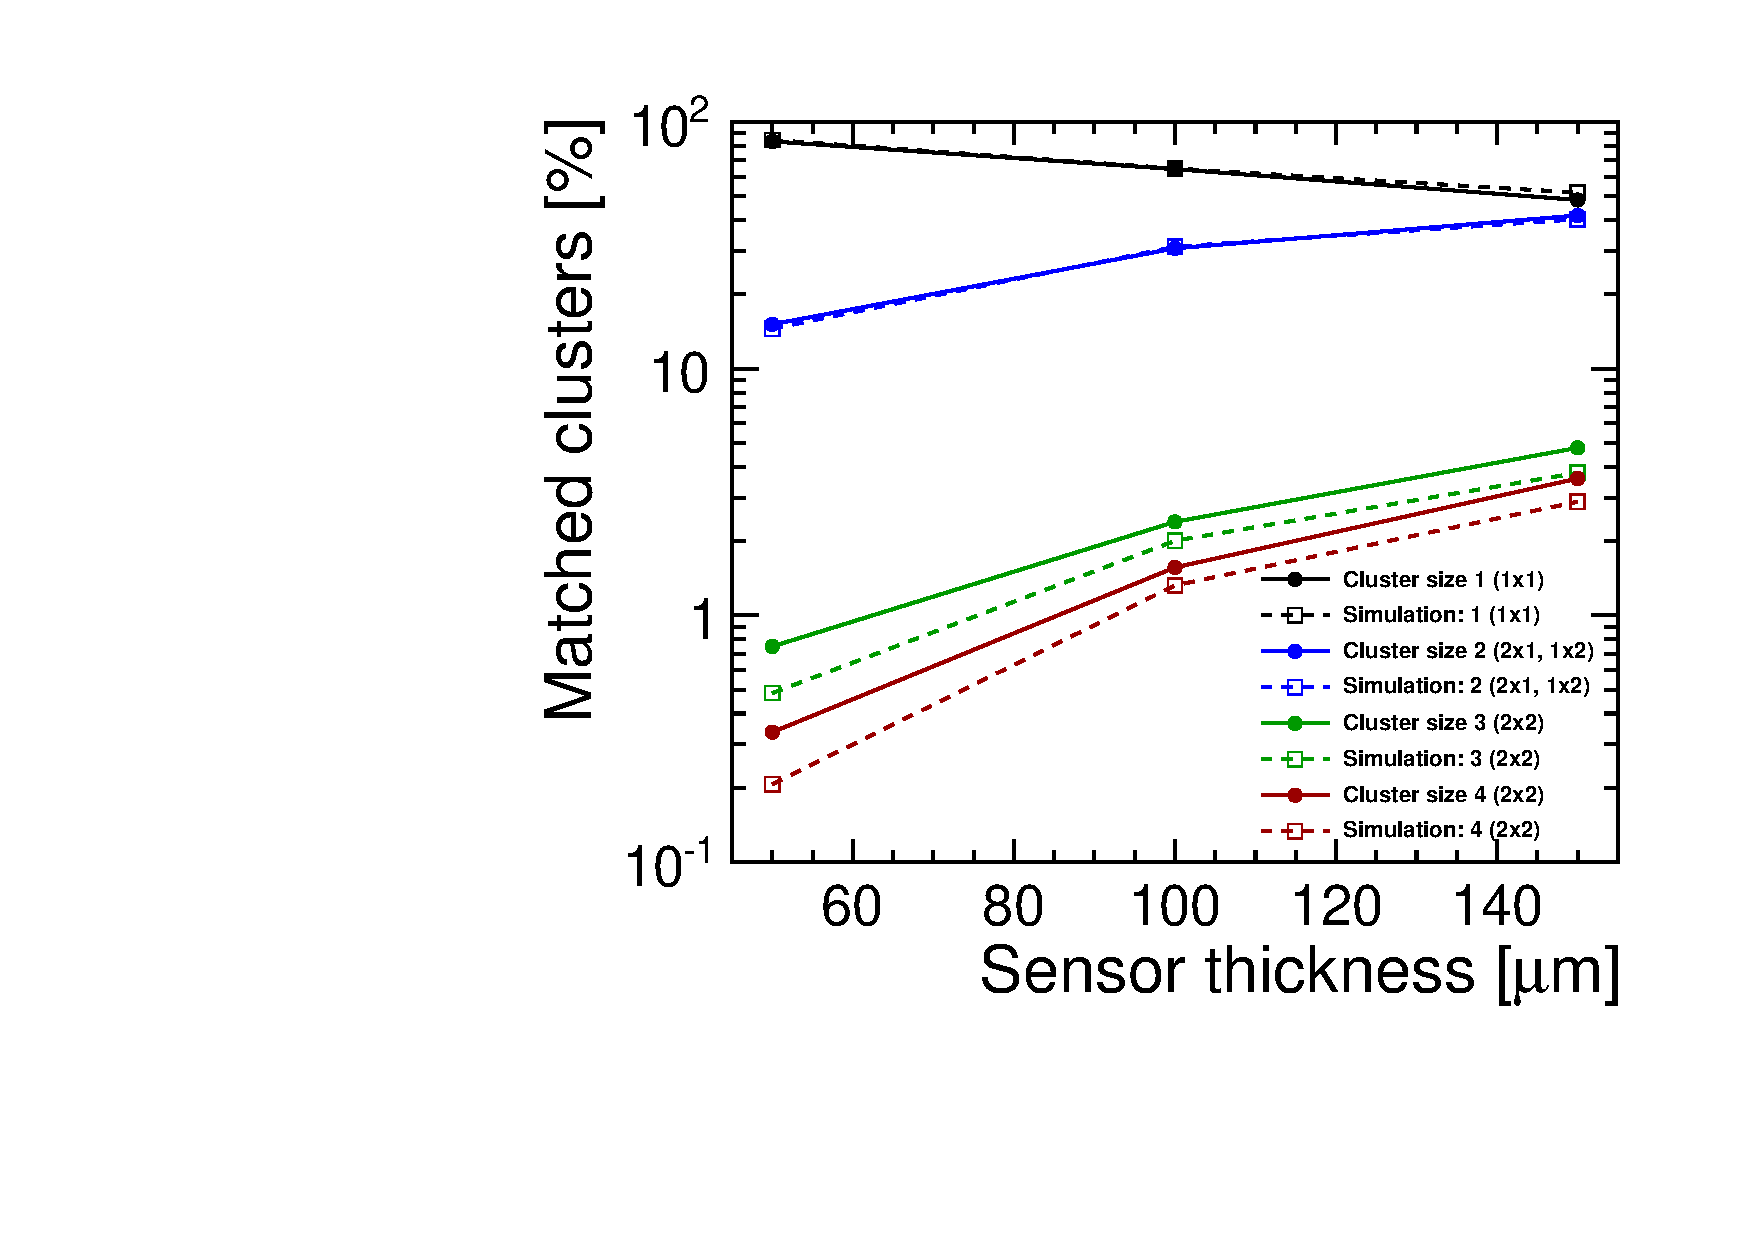
\includegraphics[width=\textwidth]{../figures/TestBeam/cluSize_vs_thickness.pdf}

    \column{0.5\textwidth}
    \centering
    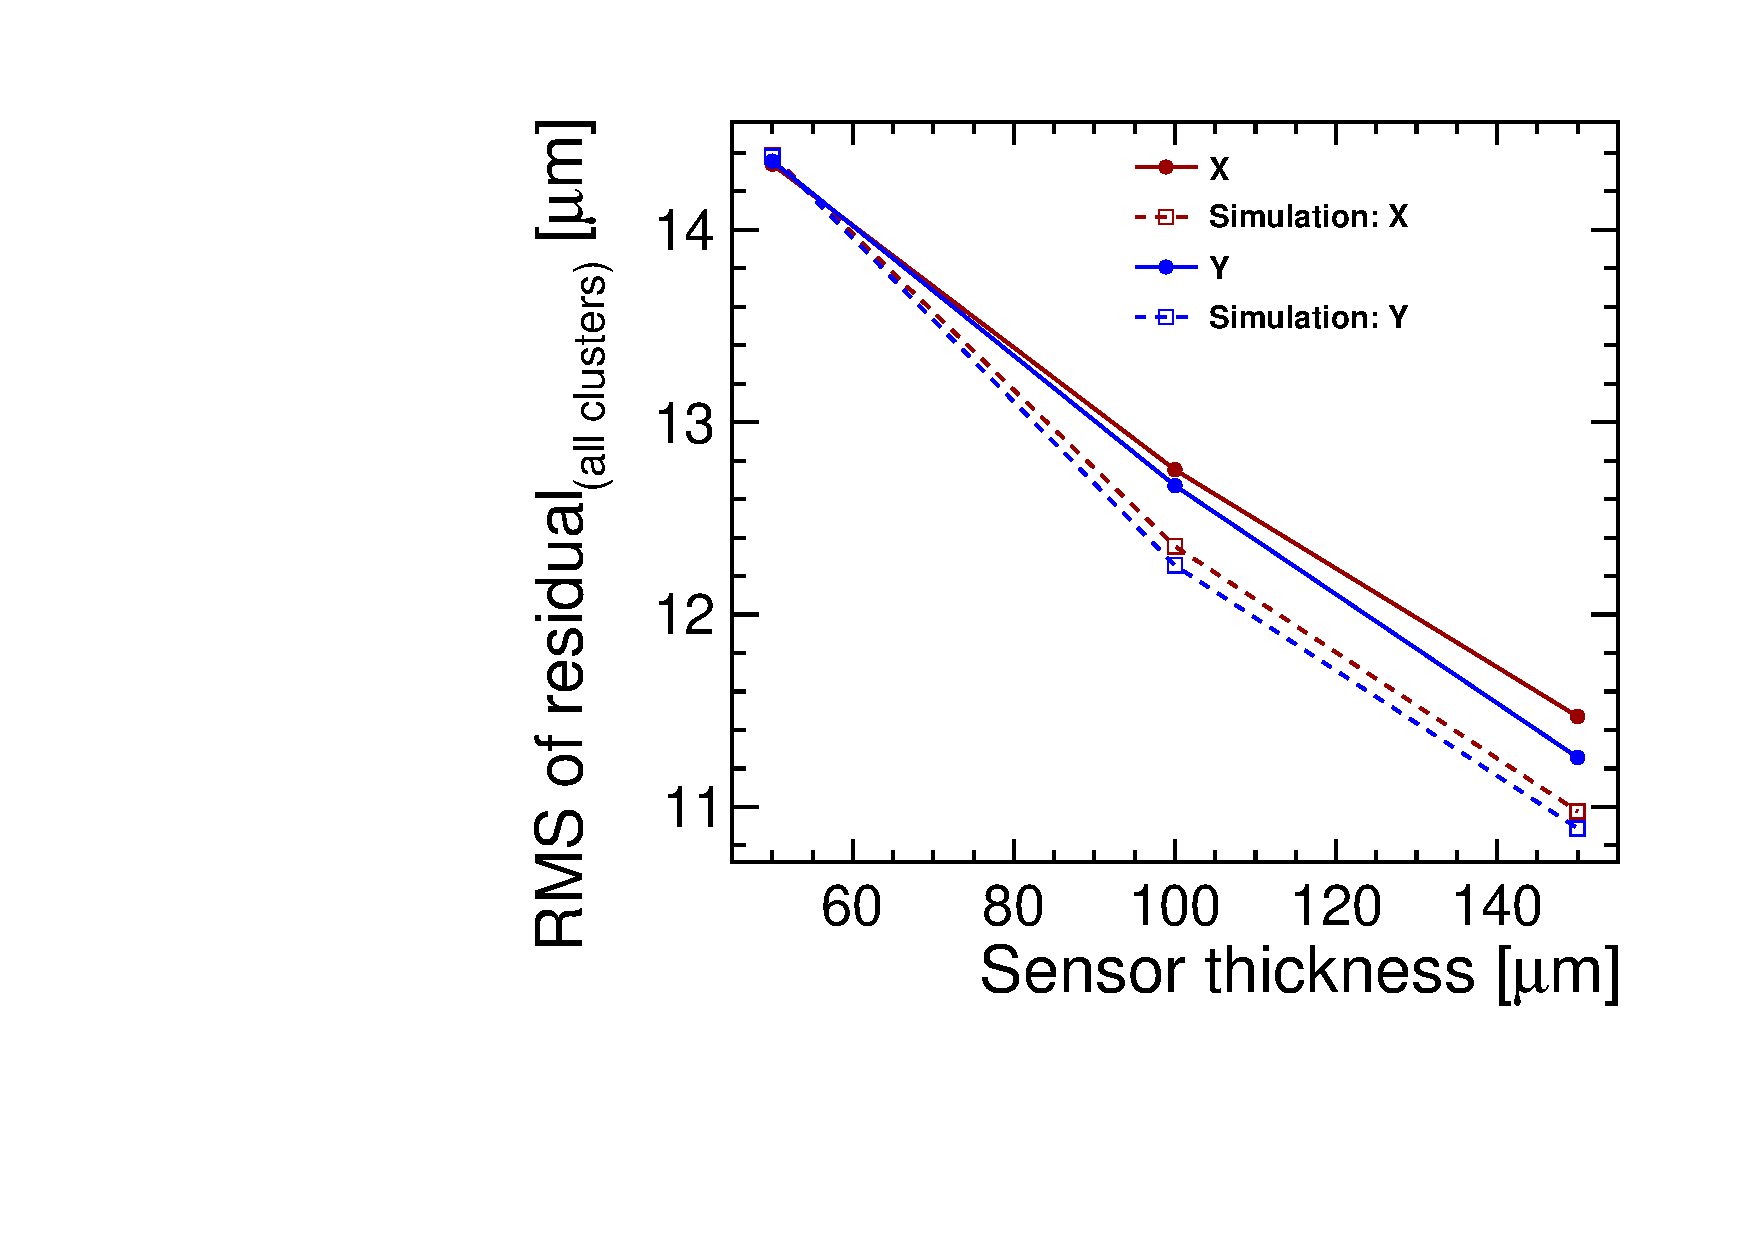
\includegraphics[width=\textwidth]{../figures/TestBeam/residuals_vs_thickness.pdf}
  \end{columns}

\end{frame}
%%%%%%%%%%%%%%%%%%%%%%%%%%%%%
%         SLIDE             %
%%%%%%%%%%%%%%%%%%%%%%%%%%%%%
\begin{frame}
  \frametitle{Small pitch R\&D and extrapolation}


  \begin{itemize}
  \item Small-pitch ASIC R\&D:
    \begin{itemize}
    \item CLICpix readout ASIC demonstrator
    \item Matrix of $64\times64$ pixels, $25\,\micron$ pixel pitch.
    \item 65~nm CMOS technology
    \item Simultaneous measurement of time (TOA) and energy (TOT) per
      pixel.
    \item Compatible with power pulsing scheme.
    \end{itemize}
  \end{itemize}

  \begin{columns}
    \column{0.5\textwidth}
    \centering
    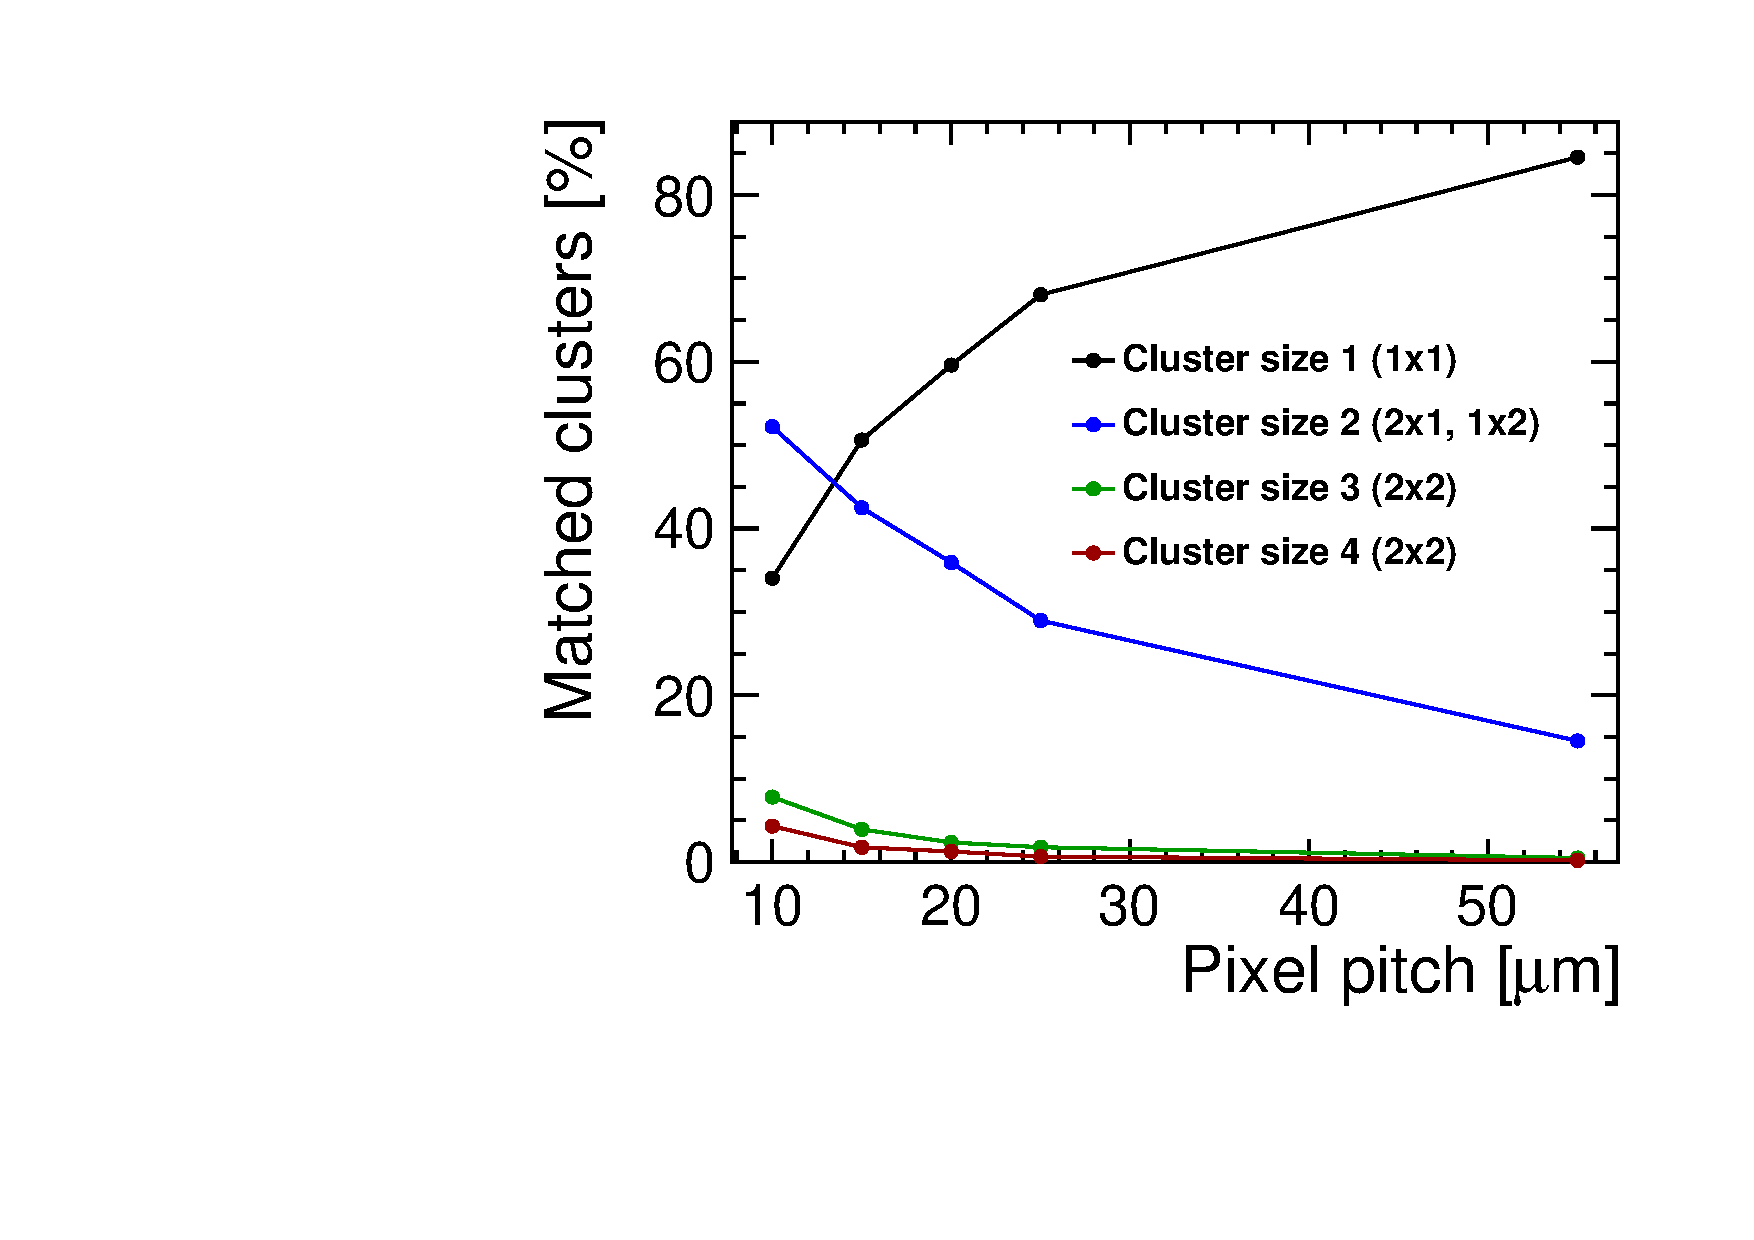
\includegraphics[width=\textwidth]{../figures/TestBeam/ClusterSize_extrapolationSmallerPixels.pdf}

    \column{0.5\textwidth}
    \centering
    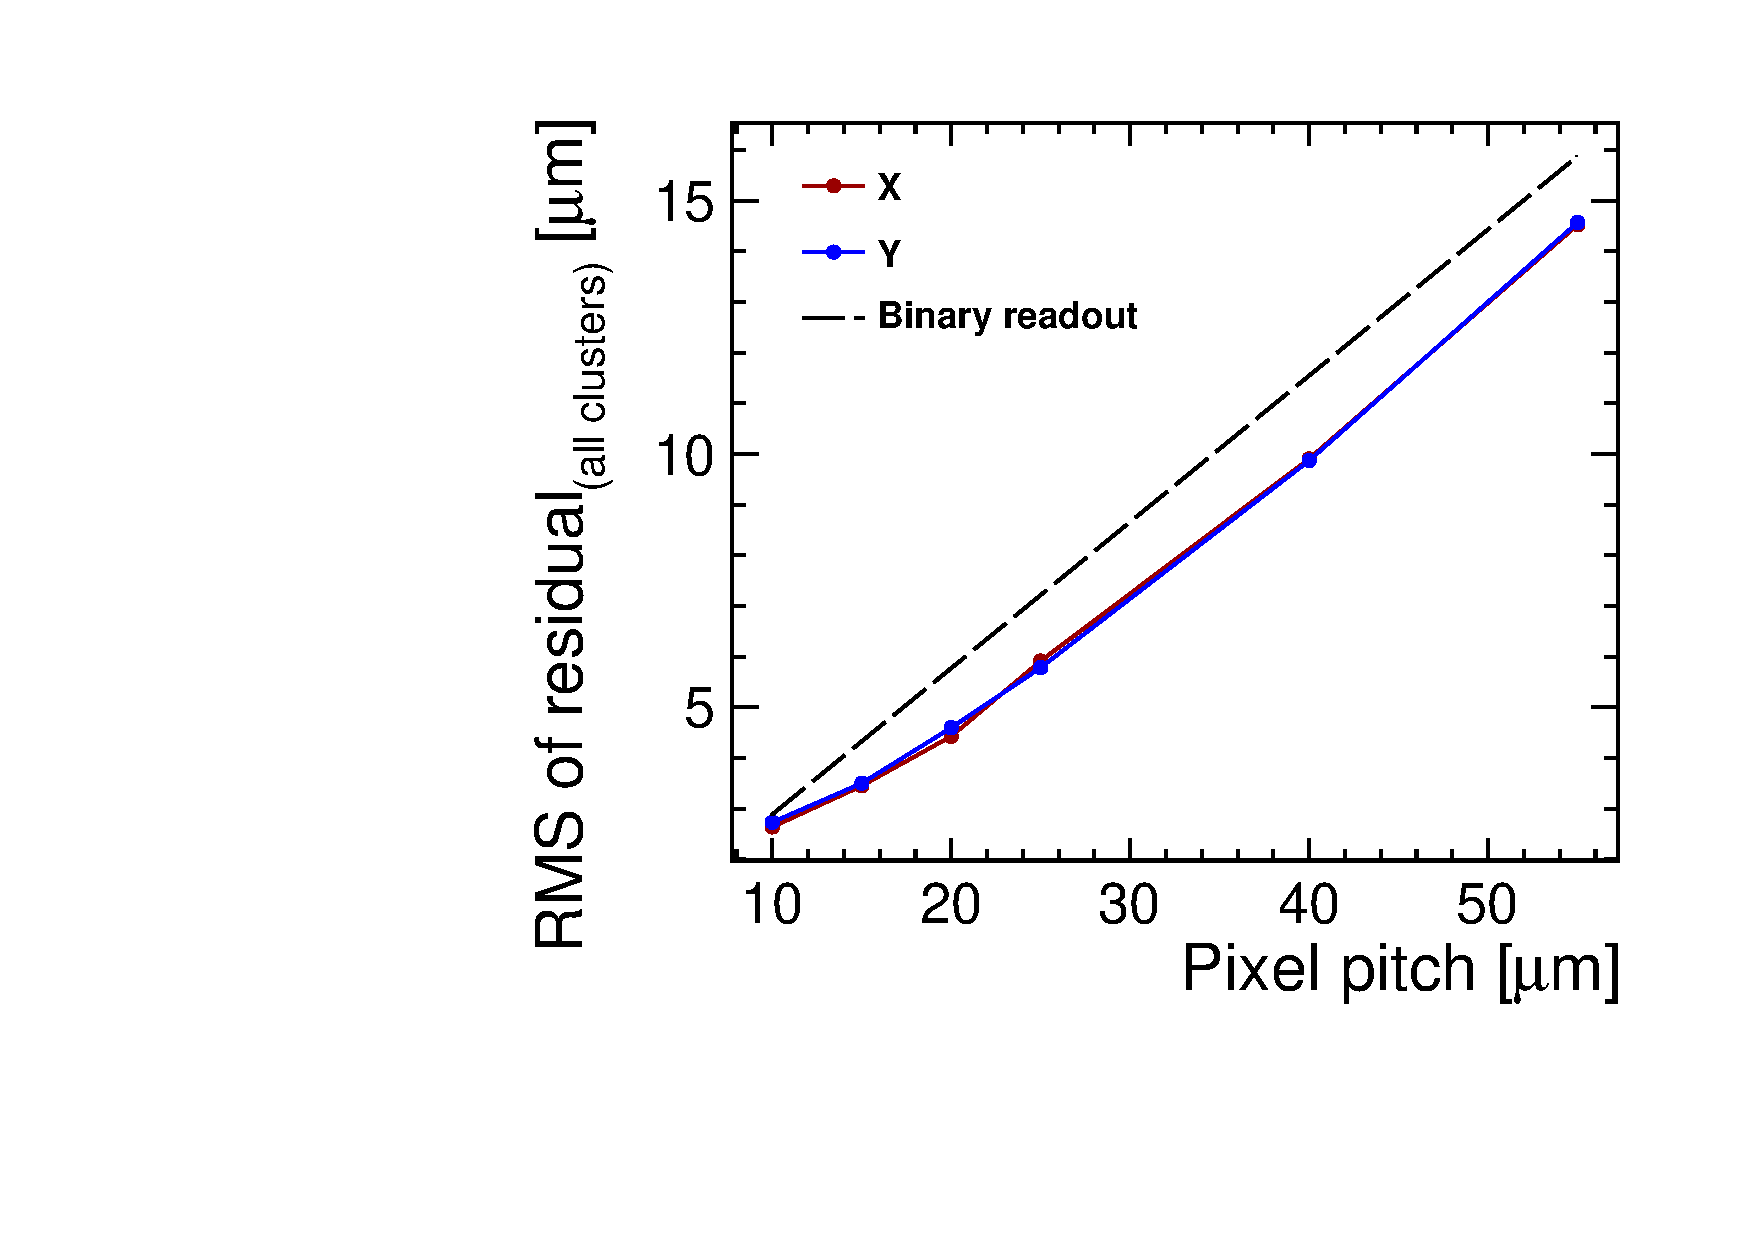
\includegraphics[width=\textwidth]{../figures/TestBeam/RMS_extrapolationSmallerPixels.pdf}
  \end{columns}

\end{frame}

%%%%%%%%%%%%%%%%%%%%%%%%%%%%%
%         SLIDE             %
%%%%%%%%%%%%%%%%%%%%%%%%%%%%%
\begin{frame}
  \frametitle{Active-edge sensors}

  \begin{itemize}
  \item The \textcolor{Blue}{DRIE} (Deep Reactive-Ion Etching) process
    is used to cut an active-edge silicon sensor.
  \item Implantation on the sidewall of the sensor $\Rightarrow$
    control the potential at the edge by creating an extension of the
    backside electrode on the edge.
  \item Guard-rings: metal and n-implants to establish a smooth
    voltage drop between the edge and the last pixel.
  \end{itemize}

  \begin{columns}

    \column{0.5\textwidth}
    \centering
    \begin{tikzpicture}
      \node[anchor=south west,inner sep=0] (image) at 
      (0,0){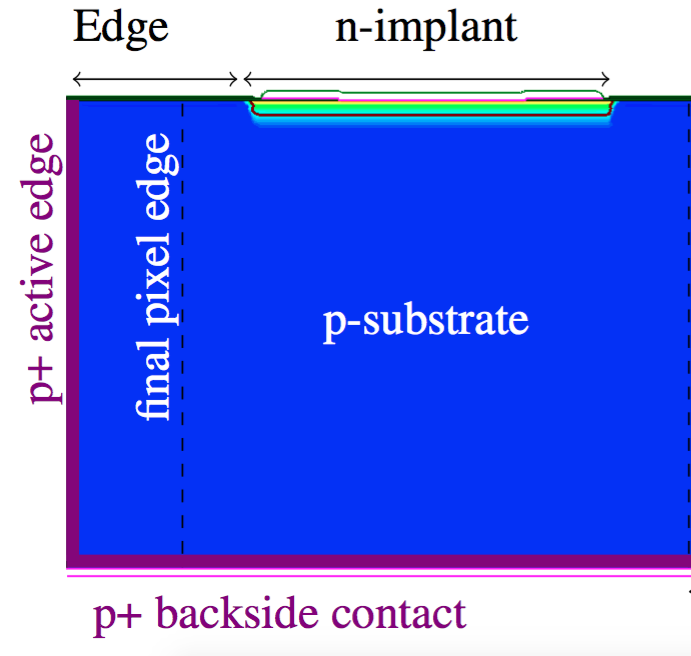
\includegraphics[width=\textwidth]{figures/EdgeSchematicTCAD_cut.png}};
      \begin{scope}[x={(image.south east)},y={(image.north west)}]
        \node[above, color=white] at (0.51, 0.1) {\small{\textbf{No guard-ring}}};
      \end{scope}
    \end{tikzpicture}
    
    \column{0.5\textwidth}
    \centering
    \begin{tikzpicture}
      \node[anchor=south west,inner sep=0] (image) at 
      (0,0){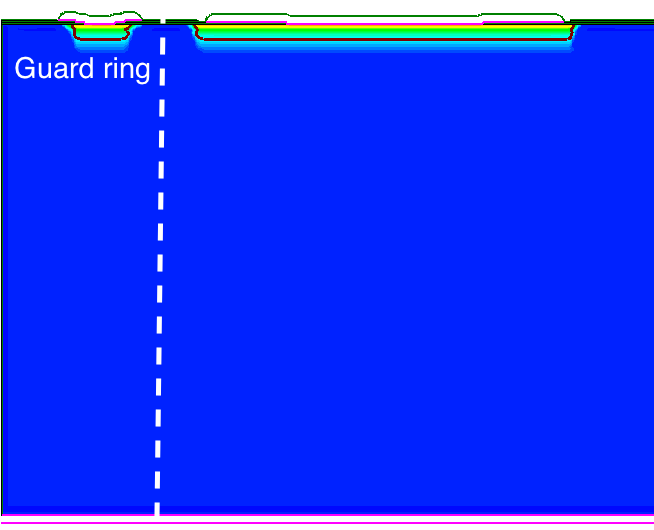
\includegraphics[width=0.85\textwidth]{figures/edgeSchematicTCAD_GuardRing_cut.png}};
      \begin{scope}[x={(image.south east)},y={(image.north west)}]
        \node[above, color=white] at (0.51, 0.1) {\small{\textbf{With guard-ring}}};
      \end{scope}
    \end{tikzpicture}
  \end{columns}



  \begin{itemize}
  \item Advacam active-edge devices (n-in-p) bump-bonded to the Timepix3 ASICs:
  \end{itemize}
  \centering
  \resizebox{\textwidth}{!}{\begin{tabular}{lccc}
      \toprule
      Assembly & Sensor thickness [\si{\micro\meter}] & Edge width
      [\si{\micro\meter}] & Edge type\\
      \midrule
      20-NGR & 50 & 20 & No guard-ring \\ %20-256
      20-FGR & 50 & 20 & Floating guard-ring \\ %20 G256
      20-GNDGR & 50 & 20 & Grounded guard-ring \\ %20-GR257
      50-GNDGR & 50 & 50 & Grounded guard-ring \\ %50-GR257
      \bottomrule
  \end{tabular}}
\end{frame}

%%%%%%%%%%%%%%%%%%%%%%%%%%%%%
%         SLIDE             %
%%%%%%%%%%%%%%%%%%%%%%%%%%%%%
\begin{frame}
  \frametitle{20-NGR-50}

  \begin{columns}
    \column{0.5\textwidth}

    \begin{itemize}
    \item Efficient up to the physical edge.
    \item All the streamlines reach the pixel.
    \end{itemize}

    \centering
    \reflectbox{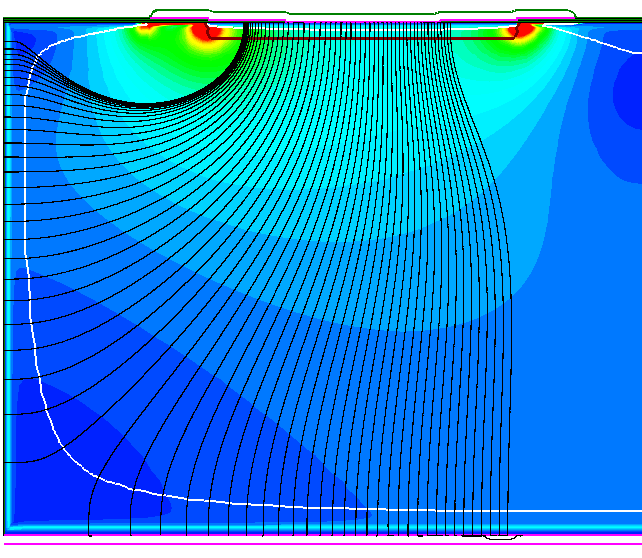
\includegraphics[width=0.3\textwidth]{../figures/ActiveEdge/streamlines_20-NGR-50.png}}

    \column{0.3\textwidth}
    \centering
    \begin{tikzpicture}
      \node[anchor=south west,inner sep=0] (image) at
      (0,0){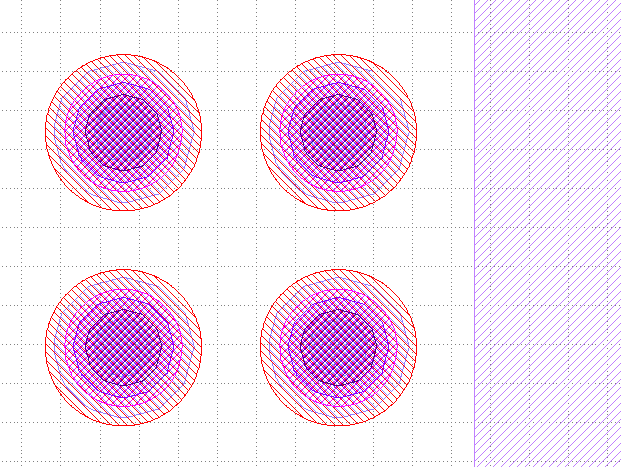
\includegraphics[width=0.8\textwidth]{figures/Layout2Pixels2.png}};
      \begin{scope}[x={(image.south east)},y={(image.north west)}]
        \node[above, color=Blue, rotate=90] at (0.1, 0.5)
        {\small{\textbf{20-NGR}}};
        \node[above, color=Blue, rotate=90] at (0.25, 0.5) {\small{(no GR)}};
        \node[above] at (0.8, 0.7) {\small{\SI{15}{\micro\meter}}};
        \draw[Blue, thick](0.765, 0.05)--(0.765, 0.95);
        \draw[Blue, thick, dashed](0.7, 0.05)--(0.7, 0.95);
        \draw[Blue, thick](0.38, 0.05)--(0.38, 0.95);
        \draw[Blue, thick](0.98, 0.05)--(0.98, 0.95);
        \draw[Blue, thick](0.38, 0.05)--(0.98, 0.05);
        \draw[Blue, thick](0.38, 0.95)--(0.98, 0.95);
        \node[below, color=Blue] at (0.38, 0.055) {-0.055};
        \node[below, color=Blue] at (0.7, 0.055) {0};
        \node[below, color=Blue] at (0.98, 0.055) {0.055};
      \end{scope}
    \end{tikzpicture}
  \end{columns}

  \begin{columns}[t]
    \column{0.5\textwidth}
    
    \begin{itemize}
    \item Efficiency vs. track position
    \end{itemize}
    \centering
    \includegraphics[width=0.8\textwidth, page=3]{../figures/TestBeam/edge_bcp.pdf}
    
    \column{0.5\textwidth}
    \begin{itemize}
    \item Energy deposition vs. track position
    \end{itemize}
    \centering
    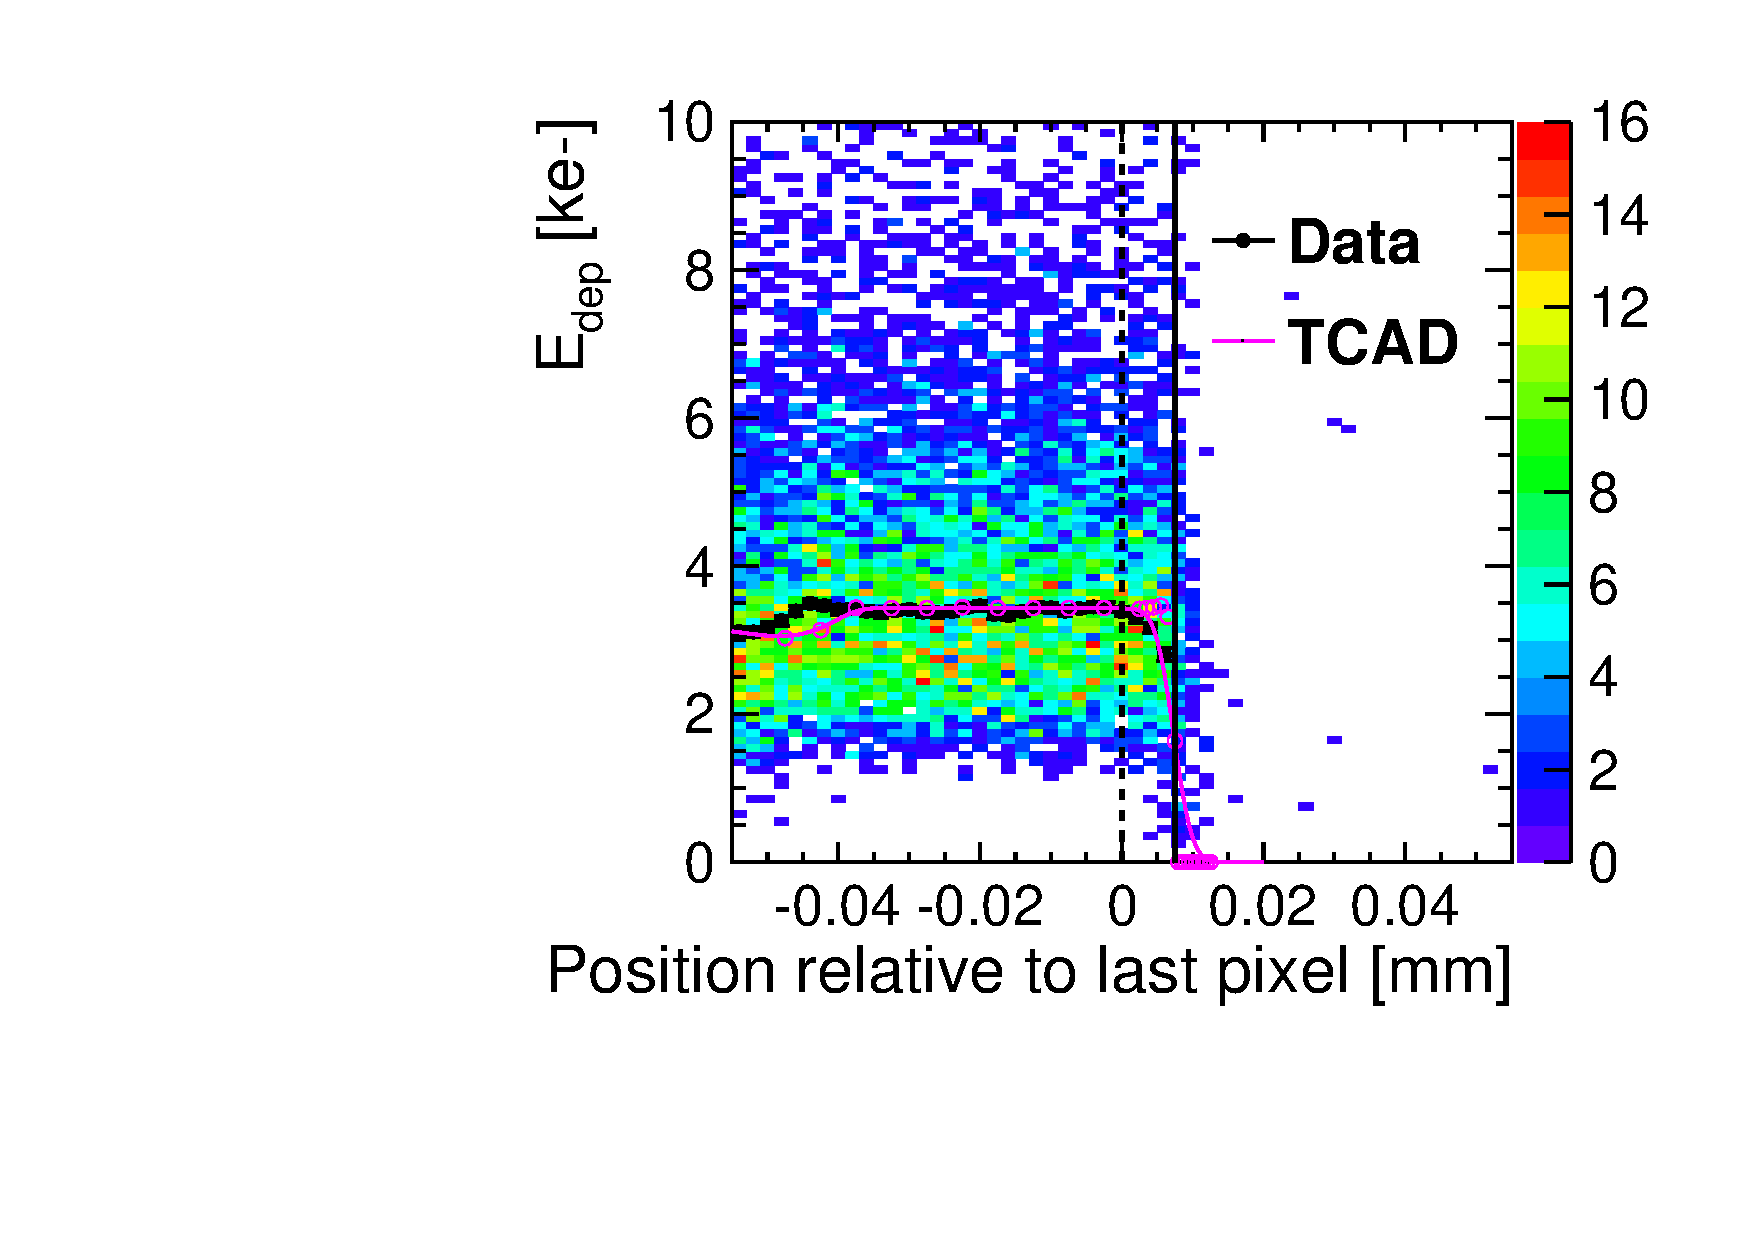
\includegraphics[width=0.8\textwidth]{../figures/ActiveEdge/20_NGR_Edep_TCAD_data.pdf}

  \end{columns}

\end{frame}


%%%%%%%%%%%%%%%%%%%%%%%%%%%%%
%         SLIDE             %
%%%%%%%%%%%%%%%%%%%%%%%%%%%%%
\label{lastslide}
\section{Conclusions}
\begin{frame}
  \frametitle{Conclusions}

  \begin{itemize}
  \item The vertex detector plays a key role to fully exploit the
    physics potential at CLIC.
    \begin{itemize}
    \item High spatial resolution (\textcolor{Blue}{$\sim3\,\micron$})
      and low material content (\textcolor{Blue}{$\sim$2\%
        X\textsubscript{0}}) $\Rightarrow$ achieve high
      flavour-tagging performance
    \end{itemize} 
    \item Characterisation of thin and active-edge planar silicon
      pixel sensors
      \begin{itemize}
      \item \textsc{Geant4} and TCAD simulations validated with
        test-beam data
      \item Extrapolation to small pixels sizes using simulations
      \item Most suitable design for active-edge designs have been
        chosen
      \end{itemize}

  \end{itemize}

\end{frame}
% %-------------------------------------------------------
% %-------------------------------------------------------
% \section{R\&D on sensor and readout technologies}
% %-------------------------------------------------------
% \subsection{Thin planar sensors}
% \begin{frame}
%   \frametitle{Thin planar sensors}
% \end{frame}
% %-------------------------------------------------------
% \subsection{The Timepix3 hybrid readout ASIC}
% \begin{frame}
%   \frametitle{The Timepix3 hybrid readout ASICs}
% \end{frame}
% %-------------------------------------------------------
% \begin{frame}
%   \frametitle{Assembly calibration}
% \end{frame}

% %-------------------------------------------------------
% %-------------------------------------------------------
% \section{Simulation}
% \begin{frame}
%   \frametitle{Simulation and reconstruction}
% \end{frame}


% %-------------------------------------------------------
% %-------------------------------------------------------
% \section{Timepix3 beam telescope}
% \begin{frame}
%   \frametitle{Timepix3 beam telescope}
% \end{frame}

% %-------------------------------------------------------
% %-------------------------------------------------------
% \section{Thin sensors studies}
% \begin{frame}
%   \frametitle{Thin sensors studies}
% \end{frame}

% %-------------------------------------------------------
% %-------------------------------------------------------
% \section{Active edge sensors}
% \begin{frame}
%   \frametitle{Active edge sensors}
% \end{frame}

% %-------------------------------------------------------
% %-------------------------------------------------------
